\documentclass[a4paper,12pt]{scrbook}
\usepackage[utf8]{inputenc}
\usepackage[slovene]{babel}
\usepackage[unicode]{hyperref}

\usepackage{amsmath}
\usepackage{amsfonts}

\usepackage{multicol}

\usepackage{enumitem}
\setlist[itemize]{itemsep=0pt, topsep=5pt}
\setlist[enumerate]{itemsep=0pt, topsep=5pt}

\usepackage[dvipsnames]{xcolor}
\usepackage{graphicx}
\usepackage{tikz}

% fonts
\usepackage[T1]{fontenc}
%\usepackage{newpxtext,newpxmath}
\usepackage{newtxtext,newtxmath}
%\usepackage{mathptmx}
%\usepackage{palatino}
%\usepackage{pxfonts}
%\usepackage{mathpazo}
%\usepackage{kpfonts}
%\usepackage{tgpagella}


% scrbook: to have the same font in headings
\setkomafont{disposition}{\bfseries}


% Okolje za pisanje nalog
%\usepackage{exercise}
\usepackage[answerdelayed]{exercise}
\renewcommand{\ExerciseHeaderTitle}{~\textit{\ExerciseTitle}~~}
\renewcommand{\ExerciseHeaderNB}{\textsf{\textbf{\thechapter.\theExercise}}}
\renewcommand{\ExerciseHeader}{\par\noindent\ExerciseHeaderNB\ExerciseHeaderTitle}
%
\renewcommand{\ExerciseSkipBefore}{5pt}
\renewcommand{\ExerciseSkipAfter}{5pt}
\renewcommand{\AnswerSkipBefore}{5pt}
\renewcommand{\AnswerSkipAfter}{5pt}


\renewcommand{\AnswerHeader}{{\par\noindent\small\ExerciseHeaderNB}~}
\renewcommand{\AtBeginAnswer}{\footnotesize}

% Bližnjice
% exercise
\def\exe#1{\begin{Exercise}#1\end{Exercise}}
% exercise: +title
\def\exetit#1#2{\begin{Exercise}[title=#1]#2\end{Exercise}}
% exercise: +label
\def\exelbl#1#2{\begin{Exercise}[label=#1]#2\end{Exercise}}
% exercise: +title, +lable
\def\exetitlbl#1#2#3{\begin{Exercise}[title=#1,label=#2]#3\end{Exercise}}
% answer
\def\ans#1{\begin{Answer}#1\end{Answer}}
% reference to the exercise 
\def\refexe#1{$\rightarrow$\ref{#1}}
% algorithm name
\def\alg#1{\quot{#1}}


% Vrste nalog - TODO:
% * zgled (naloga + rešitev + pojasnilo)
% * naloga z namigom
% * naloga z rešitvijo
% * naloga (brez dodatkov)
% * izziv (težja naloga)
% * programerska naloga
% * zanimivost (npr. Kdo je bil Evklid?)
% * raziskovalna naloga
% * "sadistična" naloga (naloga, ki pretirava z nekaterimi koncepti, npr. pointer na pointer na pointer, vendar uči "globoko" razmišljanje)


\usepackage{listings,lstautogobble}
\lstset{frame=,
	language=Pascal,
	aboveskip=1mm,
	belowskip=1mm,
	showstringspaces=false,
	columns=flexible,
	basicstyle={\small\ttfamily},
	numbers=none,
	numberstyle=\tiny\color{gray},
	keywordstyle=\color{blue},
	morekeywords={downto,return},
	commentstyle=\color{gray},
	stringstyle=\color{green},
	breaklines=true,
	breakatwhitespace=true,
	tabsize=3,
%	backgroundcolor=\color{yellow},
    autogobble=true
}

\lstnewenvironment{rox}{
	\lstset{
		mathescape=true,
		numbers=none,
		tabsize=4, 
		basicstyle=\color{Black}\small\sffamily,
		keywordstyle=\color{RoyalBlue}\small\sffamily\bfseries,
		keywords={fun,is,end,if,then,else,elif,elseif,for,to,do,while,repeat,loop,return},
	    autogobble=true
	}
}{}

% page layout
\textwidth 15cm


% % % % % % % % % % % % % % % % % % % % %

% text helpers
\def\intro#1{\par\noindent\textit{#1}\par~}
\def\angl#1{(angl. #1)}
\def\vic#1{\emph{#1}}
\def\id#1{\textsf{#1}}
\def\quot#1{''#1``}
\def\code#1{\textsf{#1}}

% math helpers
\def\NN{\ensuremath{\mathbb{N}}}
\def\ZZ{\ensuremath{\mathbb{Z}}}
\def\RR{\ensuremath{\mathbb{R}}}
\def\set#1{\{#1\}}
\def\floor#1{\lfloor#1\rfloor}
\def\ceil#1{\lceil#1\rceil}

% other 
\def\enumabc{\setlength{\itemsep}{0cm}\setlength{\parskip}{0cm}}
\def\yesno{\fbox{\begin{minipage}{0.5cm}\vspace{0.4cm}\hspace{0.5cm}\end{minipage}}\vspace{1pt}}

\renewcommand{\labelenumi}{\alph{enumi})}
\setlength{\parskip}{-0cm}


% % % % % % % % % % % % % % % % % % % % %

\makeatletter
\def\email#1{\gdef\@email{#1}}
\def\version#1{\gdef\@version{#1}}
\makeatother

\title{Vadnica iz Operacijskih sistemov}
\subtitle{(delovni osnutek, samo za interno uporabo)}
\author{Jurij Mihelič}
\email{jurij.mihelic@fri.uni-lj.si}
\version{1}
%\dedication{ads}


\begin{document}

{ % locally disable clear double page
\let\cleardoublepage\clearpage
\maketitle
\thispagestyle{empty}
\noindent
Začenjate s prebiranjem zbirke nalog za predmet \vic{Operacijski sistemi} za univerzitetni študijski program.
Gre za delovni osnutek, kar pomeni, da naloge pogosto niso dovolj dobro izpiljene in preverjene.
Prav tako besedilo verjetno vsebuje še veliko slovničnih in drugih napak.
Da študentom olajšam učenje snovi in opravljanje izpita, sem osnutek vseeno javno objavil. Želim vam mnogo prijetnih sistemskih uric.
\vfill
\noindent\rule{\textwidth}{0.4pt}\\[.5\baselineskip]
Naslov: \makeatletter\@title\makeatother\\
Različica: \makeatletter\@version\makeatother\\
Datum: \makeatletter\@date\makeatother\\[\baselineskip]
Avtor: \makeatletter\@author\makeatother\\
Elektronska pošta: \makeatletter\@email\makeatother\\[\baselineskip]
Laboratorij za algoritmiko\\
Fakulteta za računalništvo in informatiko\\
Univerza v Ljubljani\\
Večna pot 113, 1000 Ljubljana\\[\baselineskip]
\parbox{12cm}{This work is for internal purposes and is licensed under\\ Creative Commons Attribution-ShareAlike 3.0 Unported\\
(CC BY-SA 3.0).}
\hfill
\includegraphics[scale=0.6]{cc-by-sa.pdf}\\[.5\baselineskip]
\noindent\rule{\textwidth}{0.4pt}\\[\baselineskip]
\clearpage
}
\makeatother

\tableofcontents

\documentclass{book}
\usepackage{graphicx} % Required for inserting images
\usepackage[margin=1in]{geometry}

\begin{document}

\chapter{Teorija}
\section{Sistemski programi in lupina}

\begin{enumerate}
    \item Kateri dve vrsti lupin smo obravnavali glede na uporabniški vmesnik? Na kratko jih opiši.
    \item Opišite mehanizem izhodnega statusa? Katera dva sistemska klica sta povezana s tem?
    \item V ukazni lupini izvedemo ukaz mkdir a b. Koliko imeniških vnosov smo s tem ustvarili? Utemelji
    
\end{enumerate}

\section{Uporabniki, datoteke in nadzor dostopa}
aaa

\section{Upravljanje pomnilnika}
\begin{enumerate}
    \item Dan je navidezni pomnilnik z ostranjevanjem, kjer so fizični naslovi veliki N=16 bitov, navidezni naslovi M=20 bitov, odmik znotraj strani pa P=10-bitov. Kakšna je velikost deskriptorja strani, če potrebujemo poleg številke okvirja še dva bita za mehanizem varnosti? Kako velika je tabela strani in koliko pomnilnika potrebujemo za njeno shranjevanje?
    \item Opišite podobnosti in razlike priklopa datotečnih sistemov med sistemoma Windows in Linux. Kateri ukaz je namenjen temu v Linuxu?
\end{enumerate}

\section{Upravljanje procesov}
\begin{enumerate}
    \item Kaj je proces? Iz česa sestoji?
    \item Opiši izvedbo preklopa procesa.
    \item Trije procesi se sočasno izvajajo. Prvi proces najprej izpiše A nato B, drugi samo C in tretji samo D.
        \begin{enumerate}
            \item Kaj se izpiše, če se procesi na procesorju razvrstijo zaporedoma?
            \item Obrazloži, zakaj je možnih več različnih izpisov.
            \item Zapiši še vse ostale možne izpise, pri čemer izpis upoštevaj kot atomarno operacijo.
        \end{enumerate}
\end{enumerate}

\section{Medprocesna komunikacija}
\begin{enumerate}
    \item Katera sta dva osnovna načina medprocesne komunikacije? Opišite ju.
\end{enumerate}

\section{Medprocesna sinhronizacija}
\begin{enumerate}
    \item Kaj je semafor? Opiši tudi obe pripadajoči osnovni operaciji.
    \item Danih je 5 niti, ki souporabljajo spremenljivko števec, katere začetna vrednost je 0. Vsaka od niti inkrementira števec. Kakšna je lahko končna vrednost števca? Odgovor utemelji. Predpostavi LOAD/STORE arhitekturo procesorja.
    \item Opiši ukaz TEST\&SET. Kako deluje, katere lastnosti zagotavlja? Kako bi ga uporabil za izvedbo vstopa v krtični odsek?
    \item Danih je 42 procesov, ki le berejo vrednost neke skupne spremenljivke X in 6 procesov, ki vrednost skupne spremenljivke X tudi spreminjajo. Kako bi uspešno in učinkovito sinhroniziral vse te procese med seboj? Utemelji.
\end{enumerate}

\section{DA/NE vprašanja}
\begin{enumerate}
    \item Slikarski algoritem pri skladovnem upravljanju oken najprej izriše uporabniku najbližje okno.
    \item Glavna naloga mikro jedra je, da upravlja in nadzoruje mikro gonilnike.
    \item Virtualizacija sestoji iz preslikave, ki vmesnik in vire navidezne naprave preslika v vmesnik in vire realne naprave.
    \item Sistemski klic izvedemo tako, da v ustrezen register naložimo ime klica, npr. niz "fork" ali "open", nato pa izvedemo ustrezno programsko prekinitev ali namenski strojni ukaz.
    \item Operacijski sistem Linux gesla uporabniških računov hrani v datoteki /etc/passwd.
    \item Tako trde kot simbolične povezave lahko kažejo na datoteke, ki se nahajajo na drugi pomnilni napravi kot sama povezava.
    \item Sistemski klic fork() ustvari nov proces otroka, ki je kopija starša: oba imata isto kodo, različna PIDa, iste odprte datoteke in si lastita iste ključavnice.
    \item V operacijskem sistemu, ki podpira prekinjevalno večopravilnost, lahko neskončna zanka onemogoči normalno delovanje sistema.
    \item Ker exit() v celoti sprosti naslovni prostor procesa, programerju ni potrebno skrbeti za pravilno sproščanje alociranega pomnilnika.
    \item Strojni ukaz compare\&swap je posplošitev ukaza test\&set.
    \item Podatkovna struktura inode med drugim hrani tudi ime datoteke.
    \item Pri segmentaciji je pomnilnik razdeljen na bloke enake velikosti, le njihovo število je za vsak proces različno.
    \item Monitor je sinhronizacijski mehanizem, ki zagotavlja vzajemno izključevanje za vsebovane funkcije in preprečuje tudi smrtni objem.
    \item Izhodni status procesa se v operacijskem sistemu Linux hrani v procesovem deskriptorju.
    \item Mikro jedrna arhitektura operacijskega sistema v splošnem nudi boljšo varnost kot monolitna.
    \item Lupina je standardna knjižnica, ki med drugim vsebuje ovojne funkcije sistemskih klicev.
    \item Psevdo terminal je program, ki oponaša terminal tako, da omogoča vnos in prikaz podatkov kot pravi terminal.
    \item Persistenca pri datotekah pomeni, da do podatkov enotno dostopamo ne glede na dejanski fizični način njihovega hranjenja.
    \item Jedro je temeljni del operacijskega sistema in se izvaja v zaščitenem načinu procesorja.
    \item Prednost mikrojedrnih operacijskih sistemov je hitrost izvajanja, ker je izvedba mikro operacij zelo hitra.
    \item POSIX je standard, katerega namen je poenotenje funkcionalnosti UNIX-podobnih operacijskih sistemov.
    \item Uporabniški račun je mehanizem, ki vsebuje podatke o uporabniku in omogoča njihovo razlikovanje in upravljanje.
    \item Sistemski klic fork() ustvari proces tako, da mu podamo pot do izvršne datoteke, ki vsebuje strojno kodo.
    \item Pri preklopu procesa se med drugim kontekst najprej shrani v deskriptor odhajajočega procesa, nato se kontekst obnovi iz deskriptorja prihajajočega procesa.
    \item Najbolj enostaven način virtualizacije pomnilnika je, da celotno preslikovalno tabelo (za čisto vse možne navidezne naslove) hranimo v glavnem pomnilniku.
    \item Medprocesna komunikacija je mehanizem OS, ki omogoča prenos podatkov med naslovnimi prostori procesov brez kršenja zaščite procesov.
    \item Glavna naloga niti je lastništvo virov, pri čemer ima vsaka nit svoje neodvisne vire, npr. svoj pomnilnik.
    \item Pri sočasnem izvajanju lahko na enoprocesorskem sistemu pride do prepletanja izvajanja ukazov, na večprocesorskem pa tudi do njihovega prekrivanja.
    \item Za ključavnice velja, da ena nit ključavnico zaklene, druga nit jo pa odklene.
    \item Virtualizacija lahko omogoča tudi replikacijo virov, kar pomeni, da ustvarja vtis več istovrstnih naprav, kot jih dejansko je.
\end{enumerate}

\section{Ostalo}
\begin{enumerate}
    \item Kaj je randomizacija naslovnega prosta? Zakaj je koristna?
    \item V OS (npr. Linux) bomo dodali nov sistemski klic tako, da smo zanj izbrali številko 42. Vse sistemske klice od vključno 42 naprej pa smo preštevilčili (inkrementirali številko klica). Obrazloži, kaj je narobe s tem pristopom, in kako bi pravilno izvedli dodajanje sistemskega klica.
    \item Kaj je unikod? Kako kodiramo znak za novo vrstico v operacijskih sistemih Windows in Linux?
    \item Kaj je sol in zakaj se uporablja?
\end{enumerate}

\chapter{Praksa}
\section{Sistemski programi in lupina}
\begin{enumerate}
    \item Napiši skripto za lupino bash, ki rekurzivno preišče podimenike imenika, podanega kot prvi argument skripte, in iz datotek v imenom v obliki vašega AD uporabniškega imena (npr. xy1234@student.uni-lj.si) izlušči vsoto točk treh nalog. V kolikor je vsota večja ali enaka 25 točk, vsoto zapiše v skupno datoteko ucilnica.csv, ki jo skripta ustvari v imeniku, podanemu kot drugi argument programa, v obliki AD\_ime, VSOTA. V kolikor prvi argument ni podan, naj skripta privzame imenik /var/tmp. V kolikor drugi argument ni podan, naj skripta za ta imenik privzame trenutni imenik. Rekurzijo preiskovanje implementirajte sami. \\ \\ Primer datoteke xy1234@student.uni-lj.si (tocke posamezne naloge, ločene s presledki): \\10 12 9 \\ \\ Primer datoteke ucilnica.csv: \\xy1234@student.uni-lj.si, 31 \\xz2345@student.uni-lj.si, 45 
    \item Zapiši enovrstični ukaz v lupini bash, ki ugotovi in izpiše imenik, kjer se nahaja znani ukaz cat.
    \item Zapiši enovrstični ukaz v lupini bash, ki leksikografsko urejeno izpiše tretji stolpec iz datoteke /etc/passwd.
    \item Dana je spremenljivka PROCESI, ki vsebuje seznam PIDov procesov (ločeni s presledki). Zapiši enovrstični ukaz za lupino bash, ki vse procese tega seznama zaustavi za 42 sekund in nato nadaljuje njihovo izvajanje.
    \item Napišite bash skripto, ki iz datoteke, podane kot prvi argument programa (privzeta vrednost naj bo everyday.run, prebere imena ali absolutne poti programov. Za vsak program iz seznama izvede naslednje:
        \begin{itemize}
            \item Skripta naj poišče absolutno pot do programa, v kolikor je ta dosegljiv iz lupine.
            \item V primeru, da program ne obstaja v trenutnem okolju, naj skripta izpiše "ERROR: ime\_skripte" kot komentar.
            \item Skripta naj vse vrstice zapiše v datoteko zazeni.me in datoteko na koncu tudi izvede v ozadju.
        \end{itemize}
        Primer vhodne datoteke:
        \begin{verbatim}
            ls
            mkdir
            /home/student/skripta
            /home/profesor/rezultati/student/naloga1/student/resitev
            ne_obstajam
        \end{verbatim}
        Primer izpisa skripte:
        \begin{verbatim}
            /bin/usr/ls
            /bin/usr/mkdir
            /home/uporabnik/skripta
            /home/profesor/rezultati/uporabnik/naloga1/uporabnik/resitev
            #ERROR: ne_obstajam 
        \end{verbatim}
\end{enumerate}

\section{Uporabniki}
\begin{enumerate}
    \item Dana je matrika dostopa (L – lastnik, R – branje, W – pisanje, X – izvajanje):
        \begin{enumerate}
        \item Minimalno dopolni matriko:
            \begin{itemize}
                \item smiselno dodaj lastništvo
                \item uporabniki lahko berejo in pišejo vire, ki si jih lastijo
                \item uporabnik B lahko bere vse vire, razen A-jevih
                \item vir 2 lahko izvajata B in C
                \item vir 3 želimo deliti za branje in pisanje med uporabnikoma A in C \\
            \end{itemize}
            \begin{tabular}{|*{5}{p{2cm}|}}
                \hline
                Uporabnik \textbackslash Vir & 1 & 2 & 3 & 4 \\
                \hline
                A &  & R,W &  &  \\
                \hline
                B & W &  &  &  \\
                \hline
                C & R & R &  & L,R,W \\
                \hline
            \end{tabular}
        \item Zapišite nadzorni seznam dostopa (access control list), ki ga podaja dopolnjena matrika iz prejšnje točke.
    \end{enumerate}
    
\end{enumerate}

\section{Razvrščanje}
\begin{enumerate}
    \item Razvrsti procese glede na dane podatke. Nariši diagram procesov in dopolni tabelo.
        \begin{enumerate}
            \item Algoritem prvi pride, prvi mejle (FIFO) \\
                \begin{tabular}{|c|c|c|c|c|c|c|}
                    \hline
                    Proces & Dolžina & Prihodni čas & Začetni čas & Odhodni čas & Čas obdelave & Odzivni čas \\
                    \hline
                    A & 30 & 0 & & & & \\
                    \hline
                    B & 10 & 10 & & & & \\
                    \hline
                    C & 20 & 20 & & & & \\
                    \hline
                \end{tabular}
            \item Algoritem prekinjevalni najkrajši posel najprej (SJF) \\
                \begin{tabular}{|c|c|c|c|c|c|c|}
                    \hline
                    Proces & Dolžina & Prihodni čas & Začetni čas & Odhodni čas & Čas obdelave & Odzivni čas \\
                    \hline
                    A & 30 & 0 & & & & \\
                    \hline
                    B & 10 & 10 & & & & \\
                    \hline
                    C & 20 & 20 & & & & \\
                    \hline
                \end{tabular}
        \end{enumerate}
    \item Tri procese razvrščamo s prepustnicami. Prvi proces ima 10 prepustnic, drugi 20 in tretji 30. Kakšna je verjetnost izbire posameznega procesa? Kateri proces bo izbran ob žrebu prepustnice št. 15?
    \item Razvrsti procese glede na dane podatke. Uporabi časovno rezino 10 in nariši diagram procesov in dopolni tabelo.
        \begin{enumerate}
            \item Krožno ravrščanje (round robin – RR) \\
                \begin{tabular}{|c|c|c|c|c|c|c|}
                    \hline
                    Proces & Dolžina & Prihodni čas & Začetni čas & Odhodni čas & Čas obdelave & Odzivni čas \\
                    \hline
                    A & 30 & 0 & & & & \\
                    \hline
                    B & 10 & 10 & & & & \\
                    \hline
                    C & 20 & 20 & & & & \\
                    \hline
                \end{tabular}
            \item Prekinjevalni najkrajši posel najprej (preemptive shortest job first – PSJF) \\
                \begin{tabular}{|c|c|c|c|c|c|c|}
                    \hline
                    Proces & Dolžina & Prihodni čas & Začetni čas & Odhodni čas & Čas obdelave & Odzivni čas \\
                    \hline
                    A & 20 & 0 & & & & \\
                    \hline
                    B & 60 & 10 & & & & \\
                    \hline
                    C & 40 & 20 & & & & \\
                    \hline
                \end{tabular}
        \end{enumerate}
    \item Razvrsti procese glede na dane podatke. Uporabi časovno rezino 10 in nariši diagram procesov in dopolni tabelo.
        \begin{enumerate}
            \item Prvi pride, prvi melje (first come, first serve – FCFS) \\
                \begin{tabular}{|c|c|c|c|c|c|c|}
                    \hline
                    Proces & Dolžina & Prihodni čas & Začetni čas & Odhodni čas & Čas obdelave & Odzivni čas \\
                    \hline
                    A & 30 & 0 & & & & \\
                    \hline
                    B & 40 & 10 & & & & \\
                    \hline
                    C & 20 & 20 & & & & \\
                    \hline
                \end{tabular}            
            \item Prekinjevalni najkrajši posel najprej (preemptive shortest job first – PSJF) \\
                \begin{tabular}{|c|c|c|c|c|c|c|}
                    \hline
                    Proces & Dolžina & Prihodni čas & Začetni čas & Odhodni čas & Čas obdelave & Odzivni čas \\
                    \hline
                    A & 10 & 0 & & & & \\
                    \hline
                    B & 20 & 10 & & & & \\
                    \hline
                    C & 10 & 20 & & & & \\
                    \hline
                \end{tabular}
        \end{enumerate}
\end{enumerate}

\section{Jezik C}
\begin{enumerate}
    \item Napiši program v programskem jeziku C, ki naredi enako kot naslednji ukaz v lupini bash, pri čemer zunanje ukaze ustrezno zaženite (ne jih programirati): 
        \begin{verbatim}
            mkdir house && touch mouse; cat < mouse | head -42    
        \end{verbatim}
    \item Napiši program v programskem jeziku C, ki naredi enako kot naslednji ukaz v lupini bash, pri čemer zunanje ukaze ustrezno zaženite (ne jih programirati):
        \begin{verbatim}
            cat a &> out; cat out | grep error 2> error
        \end{verbatim}
    \item Za spodnji program nariši diagram izvajanja procesov, kot smo ga risali na vajah. Odgovori tudi na zastavljena vprašanja.
        \begin{enumerate}
            \item Kakšno je časovno zaporedje izhodnih statusov izvedenih procesov v programu?
            \item Kateri sistemski klici se ne izvedejo v nobenem procesu (so pa prisotni v programu)?
            \item Kaj izpiše ukaz echo \$? po izvedbi programa?
            \item Kaj procesi zapišejo na standardni izhod? Kaj izpišejo na izhod za napake?
        \end{enumerate}
        \begin{verbatim}
            int main() {
                int status = 0;
                for (int z = 0; z <= 2; z++) {
                    int a = fork();
                    if (!a) {
                        sleep(1);
                        close(1);
                        if (z == 0) {
                            printf("delam ");
                            exit(42);
                        }
                        if (z == 1) {
                            printf("se ");
                            exit(99);
                        }
                        if (z == 2) {
                            printf("da ");
                        } else {
                            printf("delam ");
                        }
                        if (z == 2) {
                            write(2, "zzz", 2);
                        }
                        sleep(z);
                        exit(z);
                    }
                    if (z == 0) {
                        waitpid(-1, &status, 0);
                        printf("cakam ");
                        exit(WEXITSTATUS(status));
                    }
                }
                exit(100);
            }
        \end{verbatim}
    \item Napiši program v programskem jeziku C, ki naredi enako kot naslednji ukaz v lupini bash, pri čemer zunanje ukaze ustrezno zaženite (ne jih programirati):
        \begin{verbatim}
            (mkdir house && touch mouse) || cat tail
        \end{verbatim}
\end{enumerate}

\section{Ostalo}
\begin{enumerate}
    \item Reši naslednjo nalogo iz stanj procesa.
        \begin{enumerate}
            \item Nariši osnovni diagram prehajanja stanj procesa. 
            \item Obrazloži prehod iz stanja izvajan v čakajoč. 
            \item Obrazloži prehod iz stanja čakajoč v pripravljen.
        \end{enumerate}
\end{enumerate}

\end{document}

\chapter{Sistemski programi in lupina}

\chapter{Uporabniki}


\chapter{Razvrščanje}

\section{Osnovna razvrščanja}

\intro{Osnovni razvrščevalni algoritmi so:
\begin{itemize}
	\item prvi pride, prvi melje (FCFS -- first come, first serve),
	\item najkrajši posel najprej (SJF -- shortest job first),
	\item prevzemni najkrajši posel najprej (PSJF -- preemptive shortest job first) in
	\item krožno razvrščanje (RR -- round robin).
\end{itemize}
}


\begin{Exercise}
Za razvrščanje procesov v spodnji tabeli uporabi algoritma a) FCFS in b) SJF:
\par\vspace{5pt}
{\centering
\begin{tabular}{r|ccccc}
	proces & A & B & C & D & E \\
	\hline
	trajanje & 10 & 20 & 30 & 40 & 50 \\
	čas prihoda & 0 & 5 & 10 & 15 & 20 \\
\end{tabular}\\}
\end{Exercise}
\ans{
Za oba FCFS in SJF je enaka razporeditev procesov. V diagramu je znotraj okvira zapisan proces in čas njegovega izvajanja, nad diagramom so procesi, kot so prihajali v sistem, pod diagramom pa je čas.
\vspace{-2em}
\begin{center}
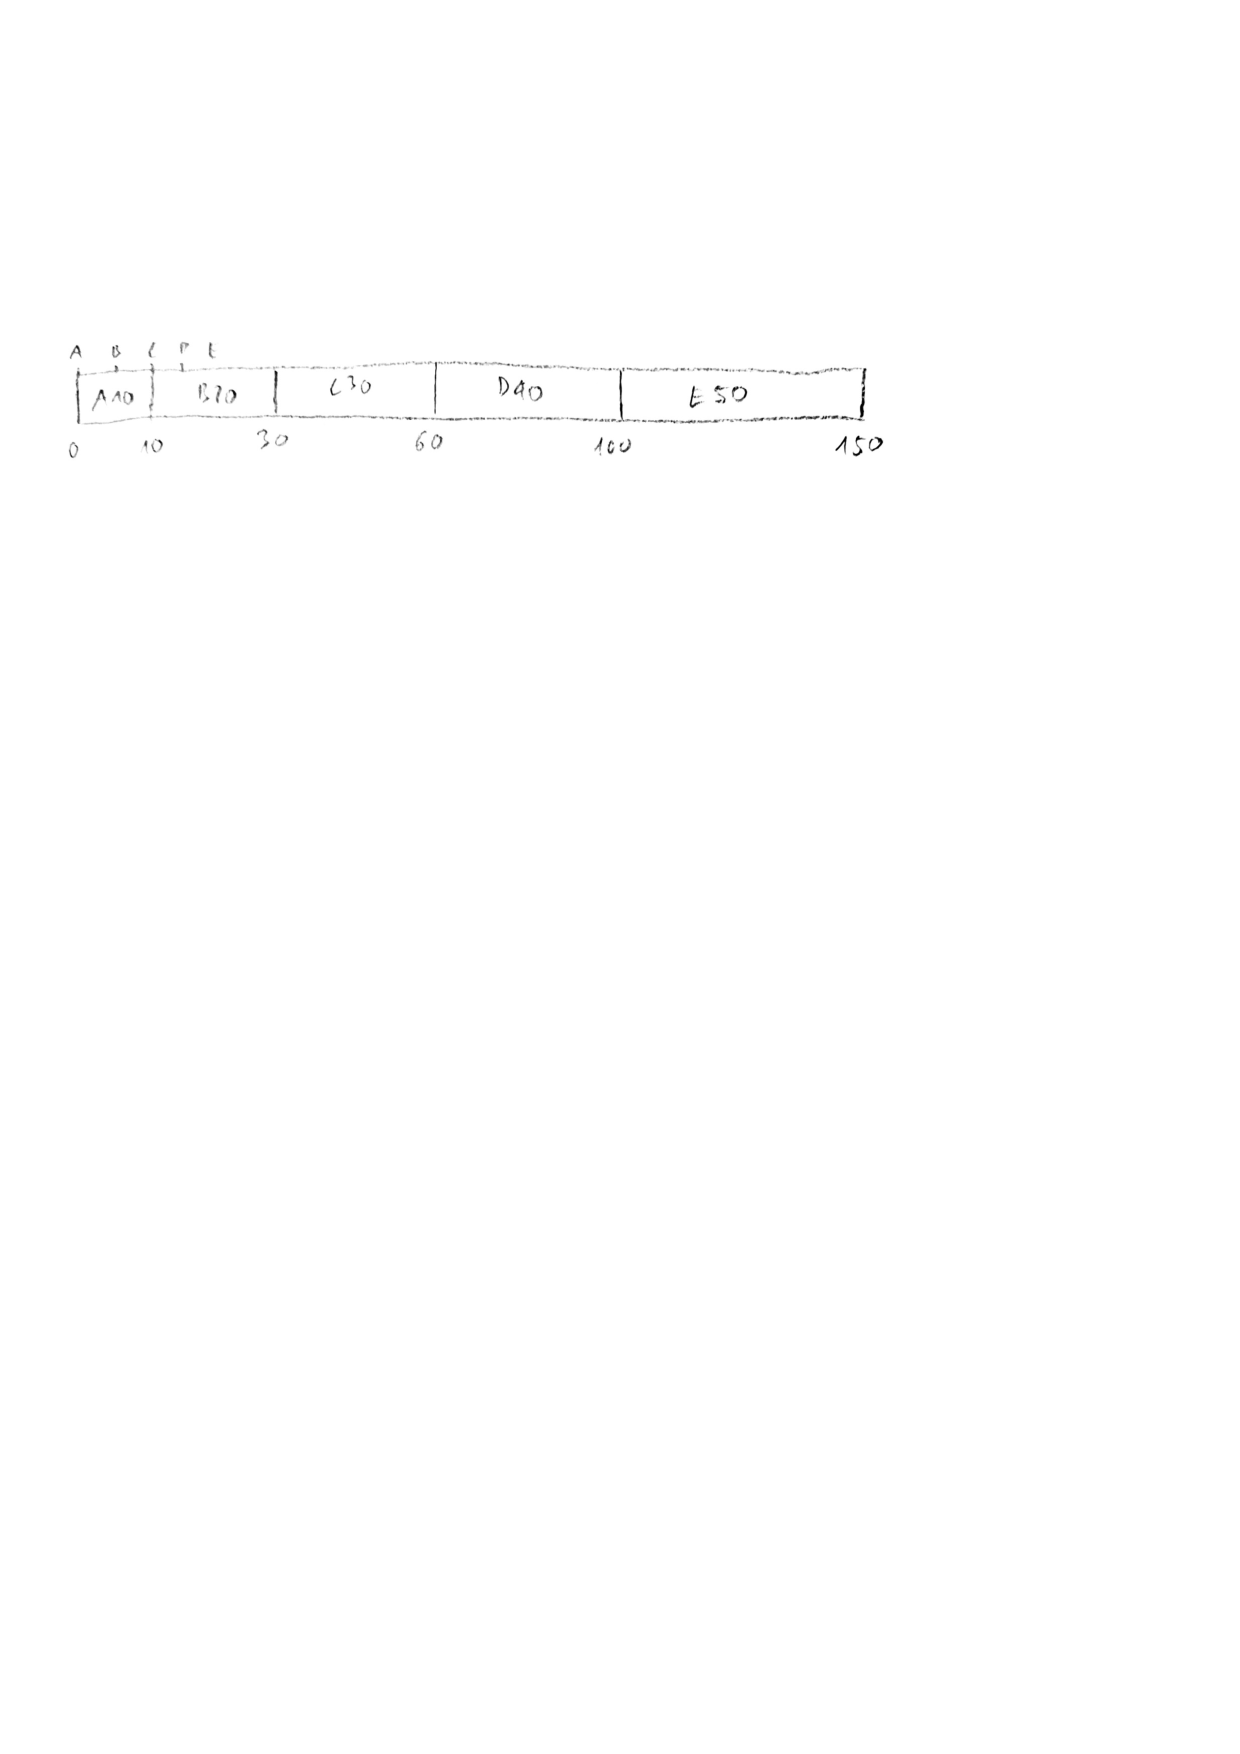
\includegraphics[width=.9\textwidth]{razvrscanje/1.1-FCFS,SJF.pdf}\\
\begin{tabular}{c|cc|cc|cc}
proces & trajanje & prihod & začetek & odhod & odzivni čas & čas obdelave \\
\hline
A & 10 &  0 &   0 & 10 & 0 & 10 \\
B & 20 &  5 & 10 & 30 & 5 & 25 \\
C & 30 & 10 & 30 & 60 & 20 & 50 \\
D & 40 & 15 & 60 & 100 & 45 & 85 \\
E & 50 & 20 & 100 & 150 & 80 & 130 \\
\hline
& & & & & 30 & 60
\end{tabular}
\end{center}
}


\begin{Exercise}
Za razvrščanje procesov v spodnji tabeli uporabi algoritma a) FCFS in b) SJF.
\par\vspace{5pt}
{\centering
\begin{tabular}{r|ccccc}
	proces & A & B & C & D & E \\
	\hline
	trajanje & 50 & 40 & 30 & 20 & 10 \\
	čas prihoda & 0 & 5 & 10 & 15 & 20 \\
\end{tabular}\\}
\end{Exercise}
\ans{
a) FCFS\\
\begin{center}
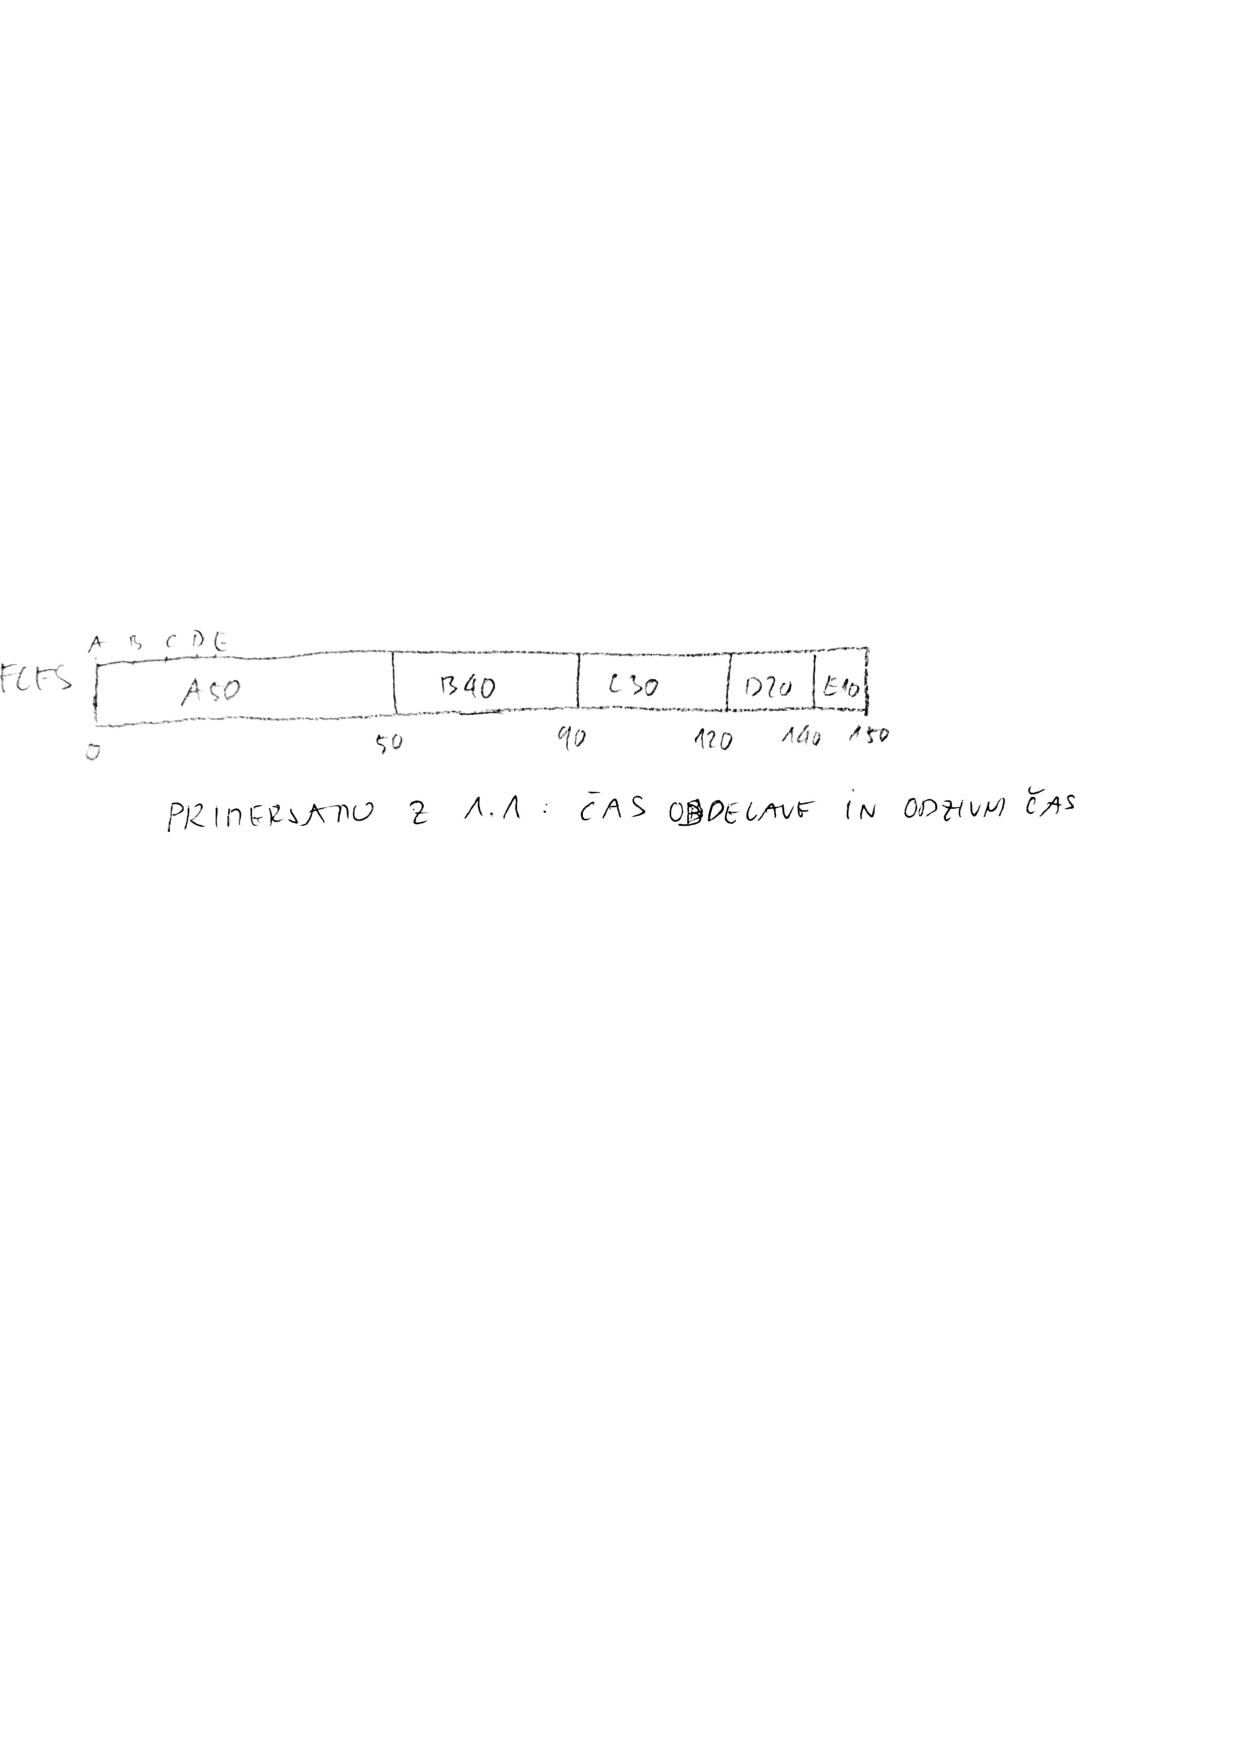
\includegraphics[width=.9\textwidth]{razvrscanje/1.2-FCFS.pdf}\\
\begin{tabular}{c|cc|cc|cc}
proces & trajanje & prihod & začetek & odhod & odzivni čas & čas obdelave \\
\hline
A & 50 &  0 &   0 & 50 & 0 & 50 \\
B & 40 &  5 & 50 & 90 & 45 & 85 \\
C & 30 & 10 & 90 & 120 & 80 & 110 \\
D & 20 & 15 & 120 & 140 & 105 & 125 \\
E & 10 & 20 & 140 & 150 & 120 & 130 \\
\hline
& & & & & 70 & 100
\end{tabular}
\end{center}
b) SJF:
\begin{center}
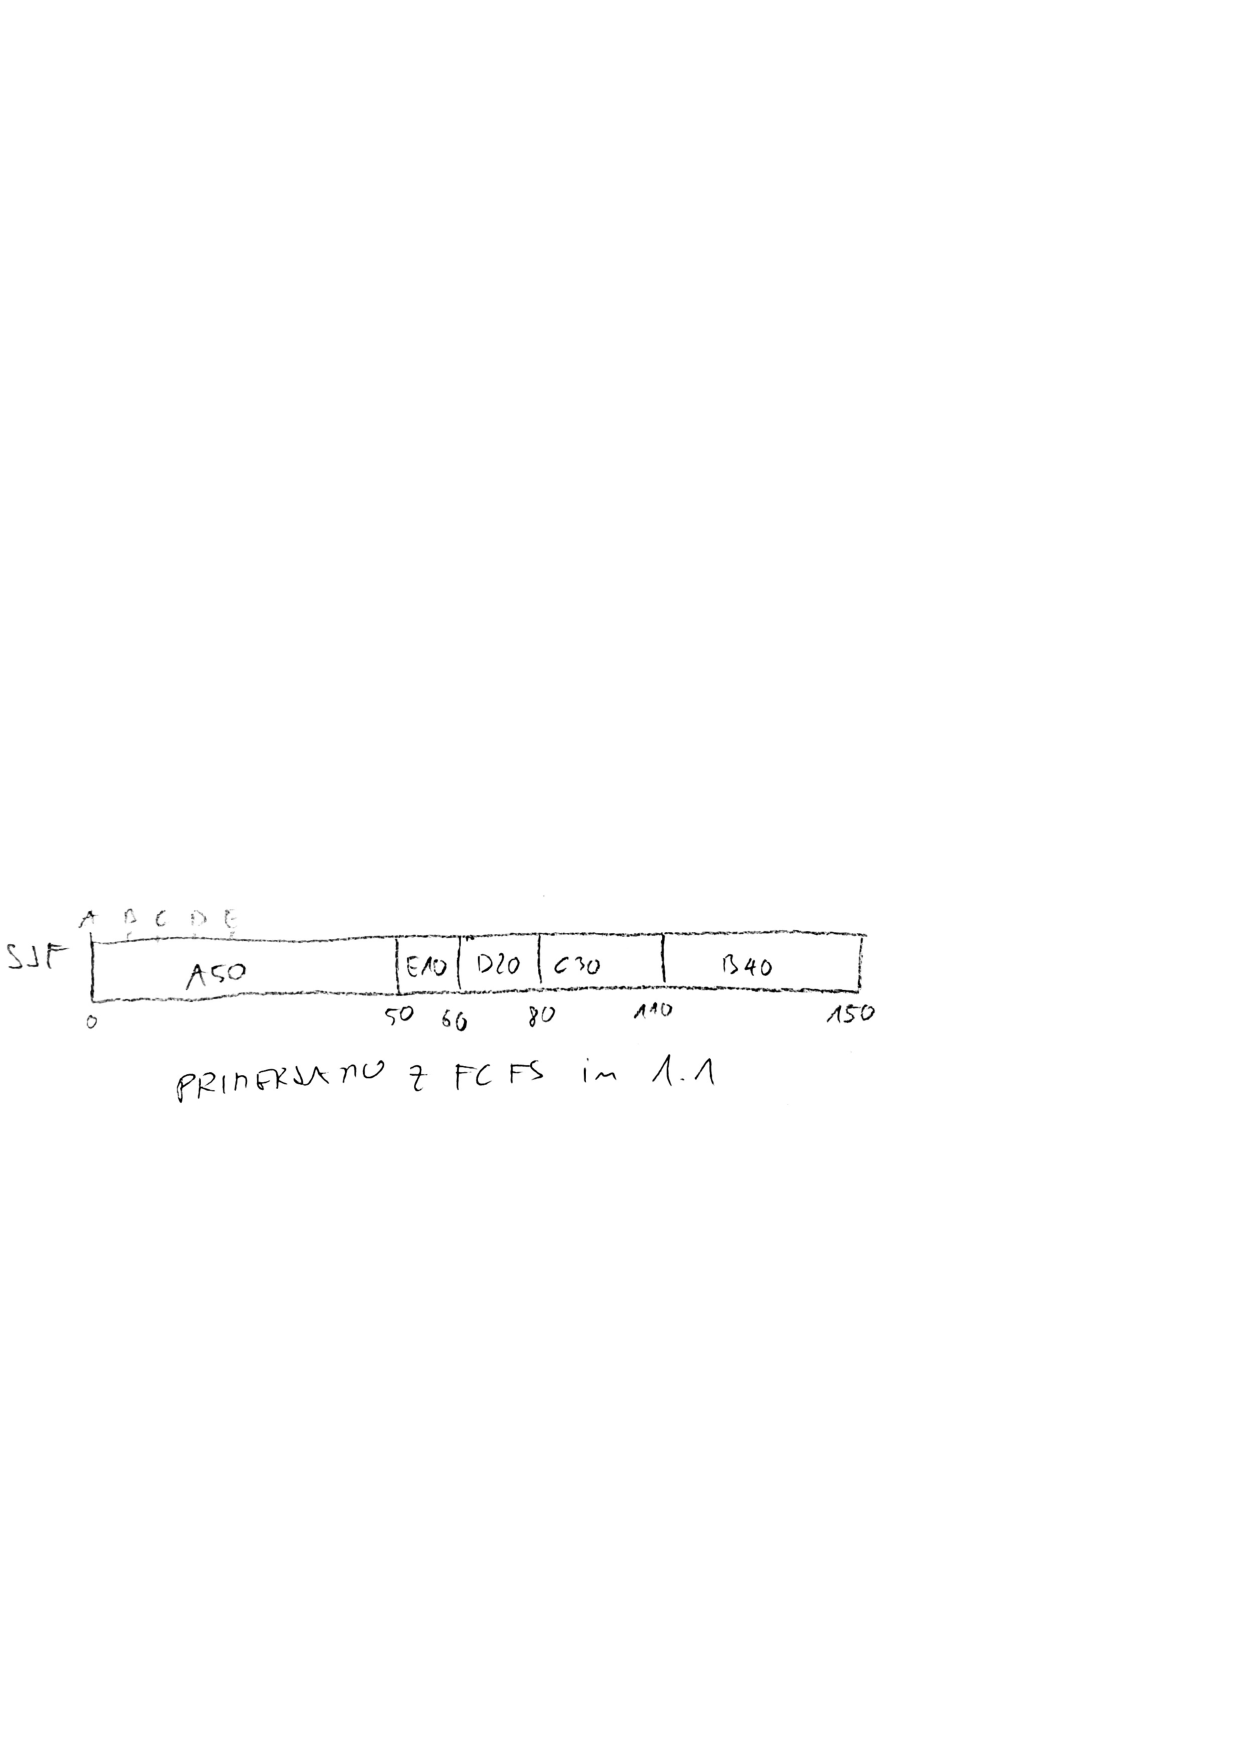
\includegraphics[width=.9\textwidth]{razvrscanje/1.2-SJF.pdf}\\
\begin{tabular}{c|cc|cc|cc}
proces & trajanje & prihod & začetek & odhod & odzivni čas & čas obdelave \\
\hline
A & 50 &  0 &   0 & 50 & 0 & 50 \\
B & 40 &  5 & 110 & 150 & 105 & 145 \\
C & 30 & 10 & 80 & 110 & 70 & 100 \\
D & 20 & 15 & 60 & 80 & 45 & 65 \\
E & 10 & 20 & 50 & 60 & 30 & 40 \\
\hline
& & & & & 50 & 80
\end{tabular}
\end{center}
}


\begin{Exercise}
Za razvrščanje procesov v spodnji tabeli uporabi algoritma a) FCFS in b) SJF.
\par\vspace{5pt}
{\centering
\begin{tabular}{r|ccccc}
	proces & A & B & C & D & E \\
	\hline
	trajanje & 10 & 30 & 30 & 10 & 20 \\
	čas prihoda & 0 & 0 & 10 & 10 & 20 \\
\end{tabular}\\}
\end{Exercise}
\ans{
a) FCFS:
\begin{center}
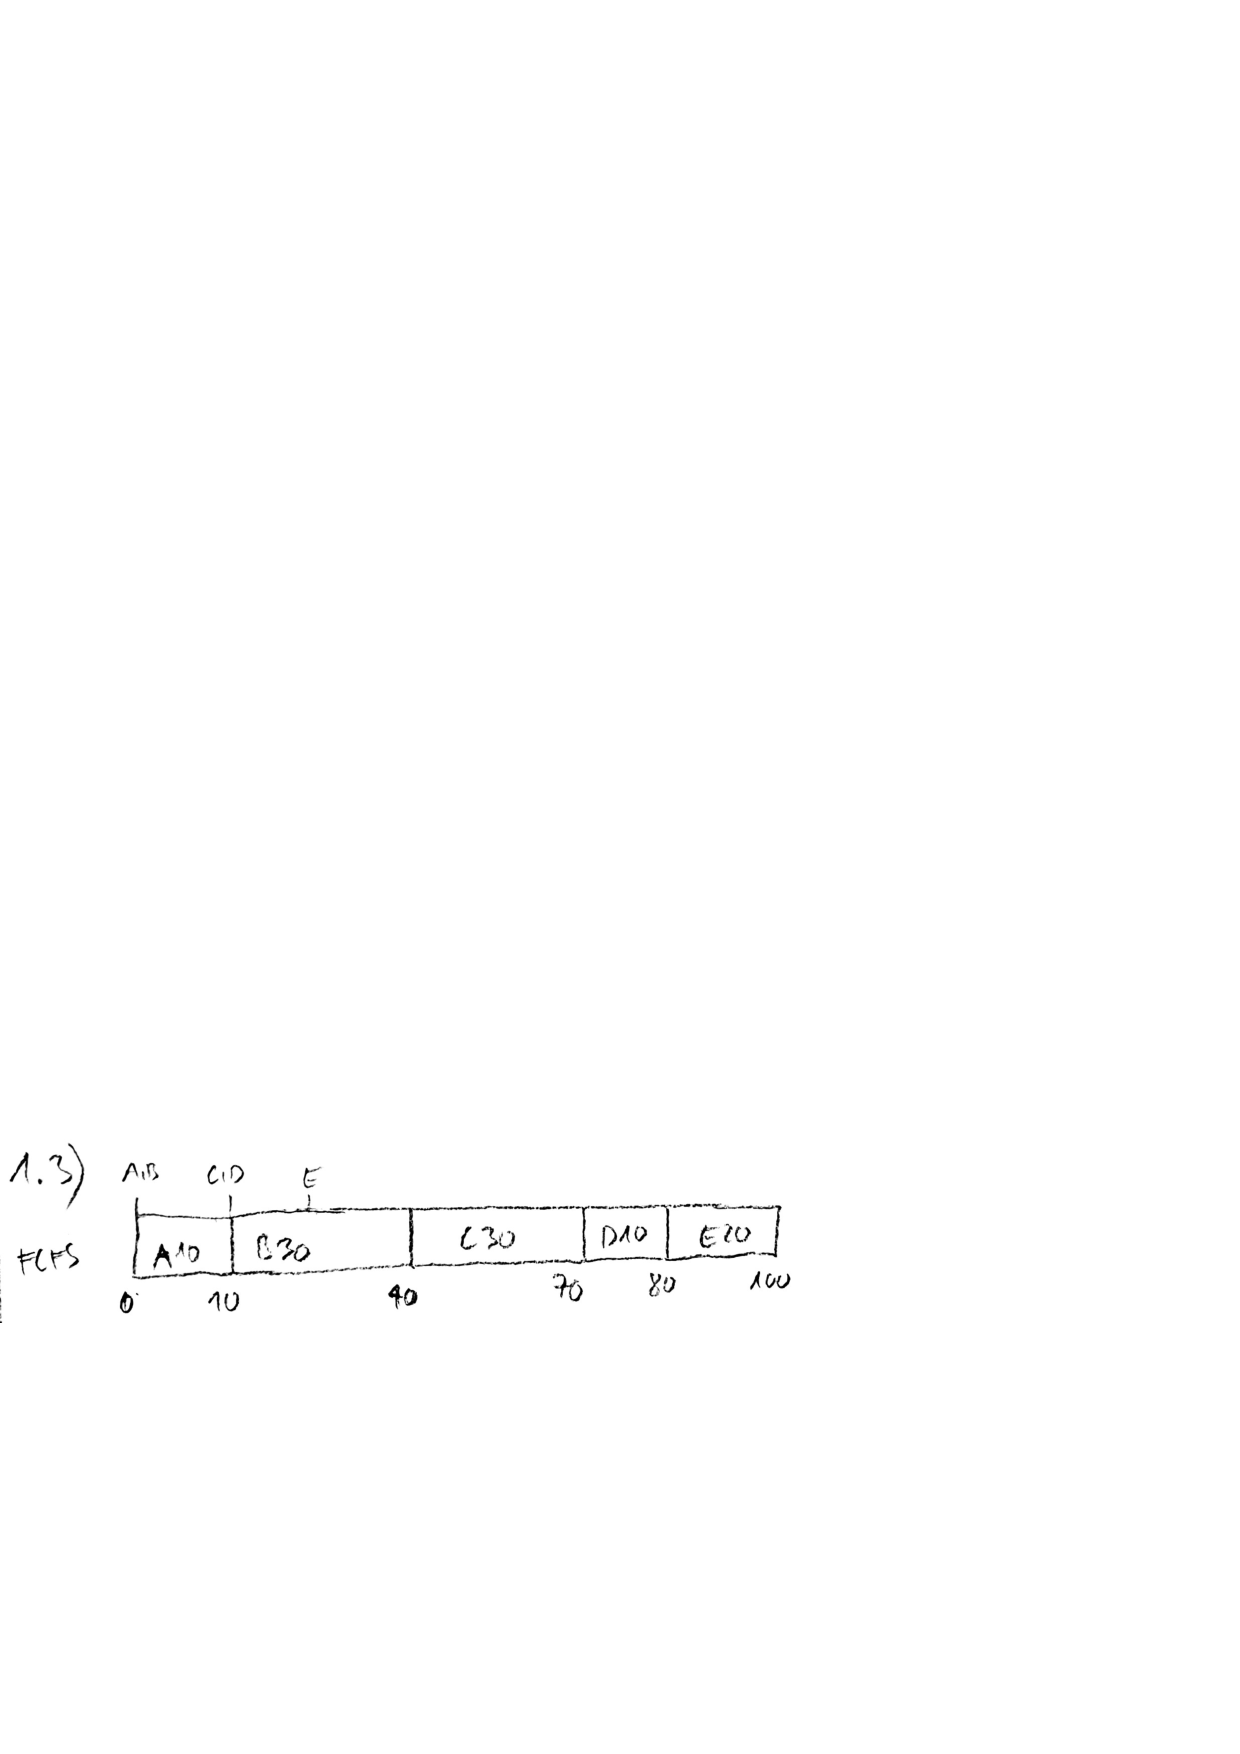
\includegraphics[width=.9\textwidth]{razvrscanje/1.3-FCFS.pdf}\\
\begin{tabular}{c|cc|cc|cc}
proces & trajanje & prihod & začetek & odhod & odzivni čas & čas obdelave \\
\hline
A & 10 &  0 &   0 & 10 & 0 & 10 \\
B & 30 &  0 & 10 & 40 & 10 & 40 \\
C & 30 & 10 & 40 & 70 & 30 & 60 \\
D & 10 & 10 & 70 & 80 & 60 & 70 \\
E & 20 & 20 & 80 & 100 & 60 & 80 \\
\hline
& & & & & 32 & 52
\end{tabular}
\end{center}
b) SJF:
\begin{center}
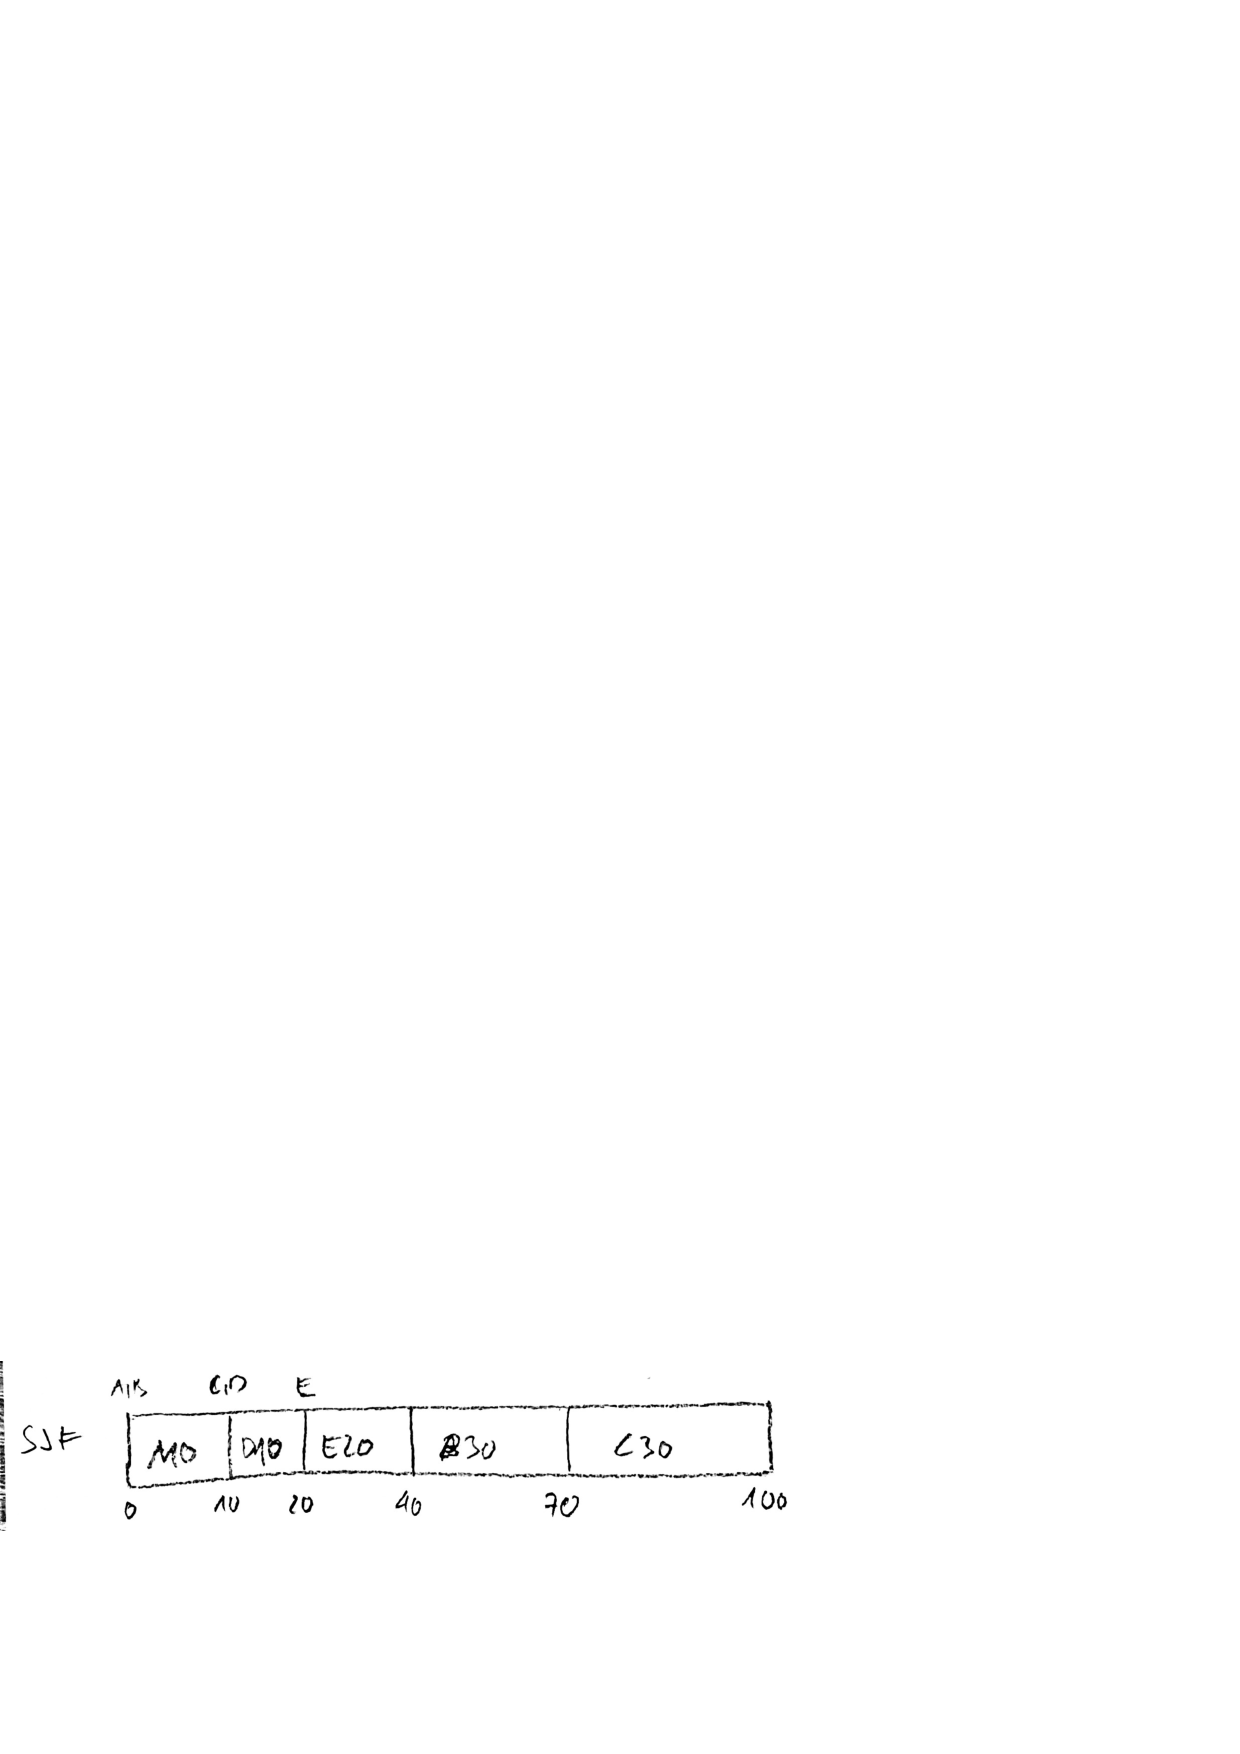
\includegraphics[width=.9\textwidth]{razvrscanje/1.3-SJF.pdf}\\
\begin{tabular}{c|cc|cc|cc}
proces & trajanje & prihod & začetek & odhod & odzivni čas & čas obdelave \\
\hline
A & 10 &  0 &   0 & 10 & 0 & 10 \\
B & 30 &  0 & 40 & 70 & 40 & 70  \\
C & 30 & 10 & 70 & 100 & 60 & 90 \\
D & 10 & 10 & 10 & 20 & 0 & 10 \\
E & 20 & 20 & 20 & 40 & 0 & 20 \\
\hline
& & & & & 20 & 40
\end{tabular}
\end{center}
}


\begin{Exercise}
Za razvrščanje procesov v spodnji tabeli uporabi algoritma a) SJF in b) PSJF.
\par\vspace{5pt}
{\centering
	\begin{tabular}{r|ccccc}
		proces & A & B & C & D & E \\
		\hline
		trajanje & 25 & 10 & 15 & 10 & 5 \\
		čas prihoda & 0 & 5 & 10 & 15 & 30 \\
	\end{tabular}\\}
\end{Exercise}
\ans{
a) SJF:
\begin{center}
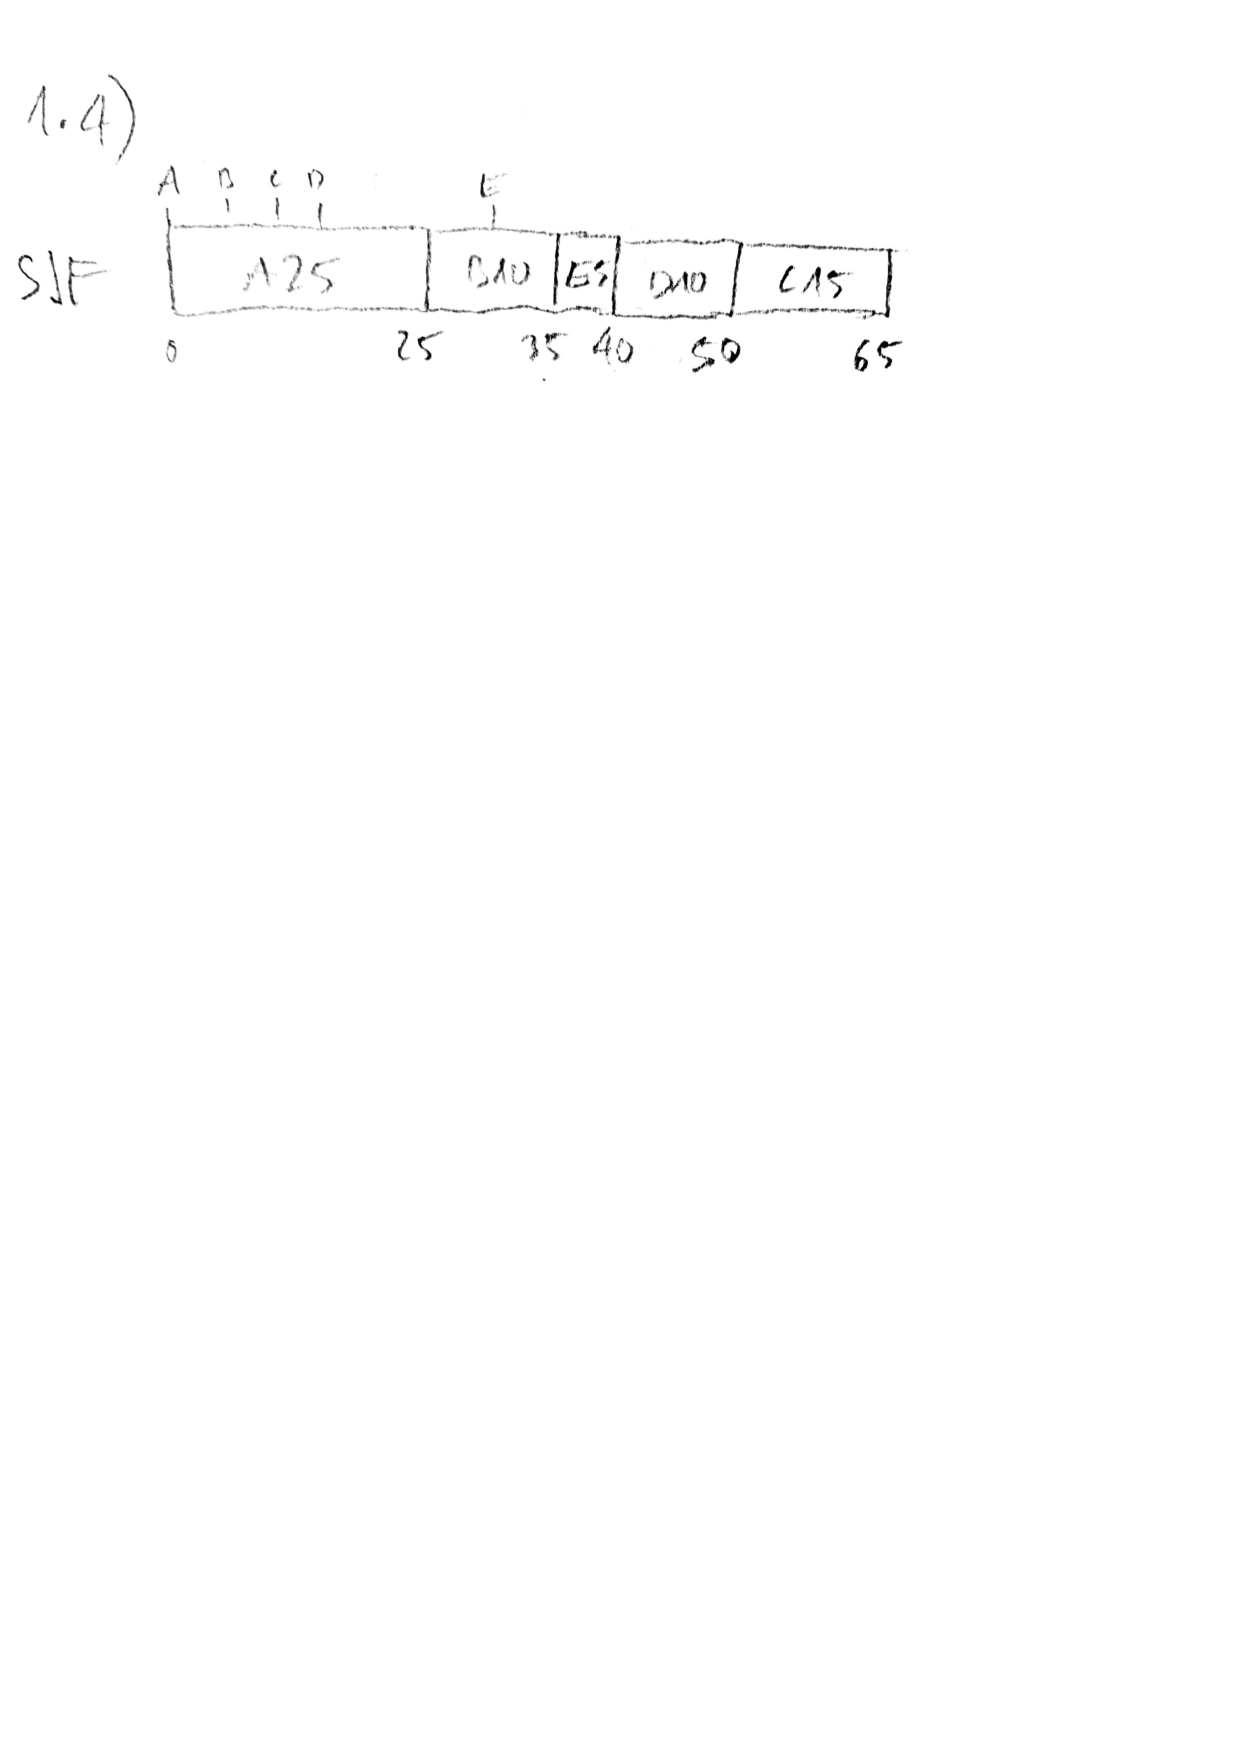
\includegraphics[width=.8\textwidth]{razvrscanje/1.4-SJF.pdf}\\
\begin{tabular}{c|cc|cc|cc}
proces & trajanje & prihod & začetek & odhod & odzivni čas & čas obdelave \\
\hline
A & 25 &  0 &   0 & 25 & 0 & 25 \\
B & 10 &  5 & 25 & 35 & 20 & 30 \\
C & 15 & 10 & 50 & 65 & 40 & 55 \\
D & 10 & 15 & 40 & 50 & 25 & 35 \\
E &  5 & 30 & 35 & 40 & 5 & 10 \\
\hline
& & & & & 18 & 31
\end{tabular}
\end{center}
b) PSJF:
\begin{center}
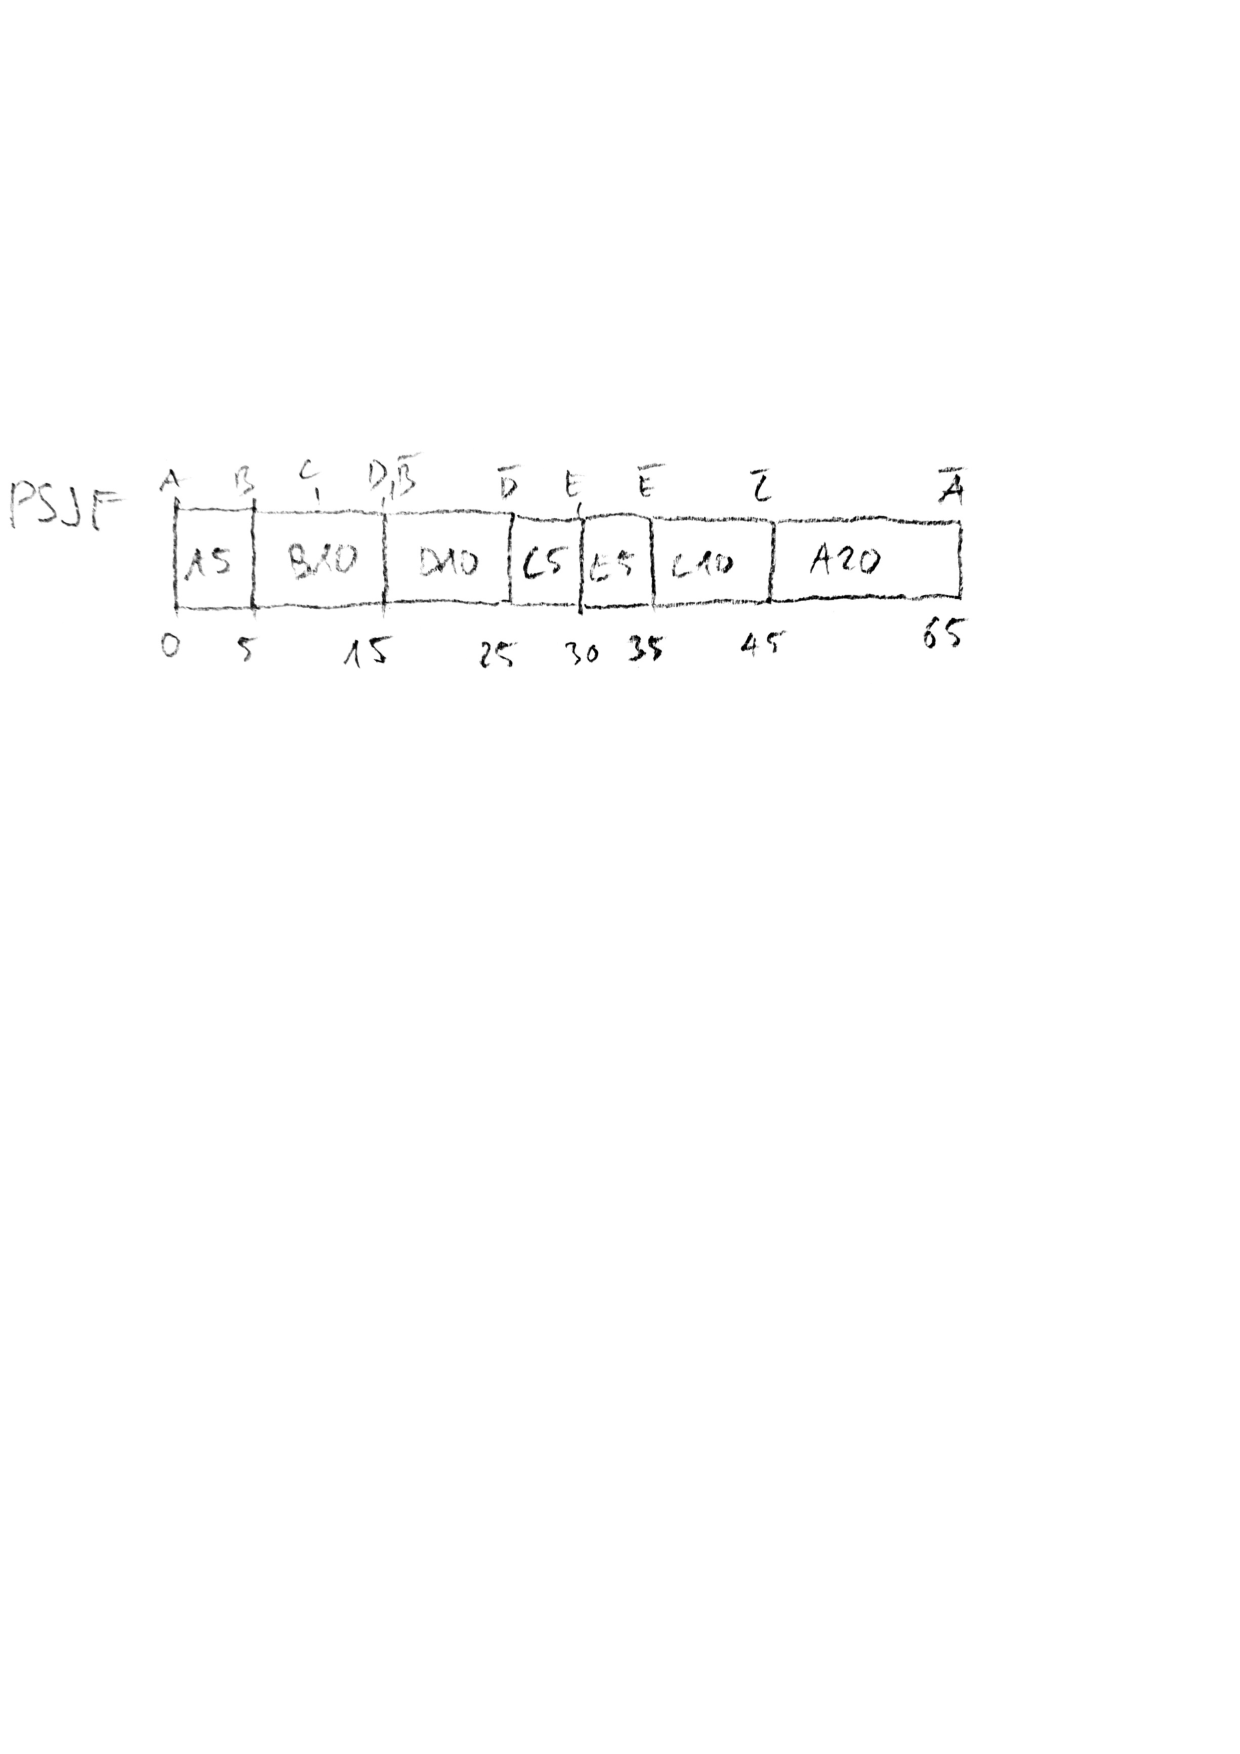
\includegraphics[width=.8\textwidth]{razvrscanje/1.4-PSJF.pdf}\\
\begin{tabular}{c|cc|cc|cc}
proces & trajanje & prihod & začetek & odhod & odzivni čas & čas obdelave \\
\hline
A & 25 &  0 &   0 & 65 & 0 & 65 \\
B & 10 &  5 &   5 & 15 &  0 & 10 \\
C & 15 & 10 & 25 & 45 & 15 & 35 \\
D & 10 & 15 & 15 & 25 & 0 & 10 \\
E &  5 & 30 & 30 & 35 & 0 & 5 \\
\hline
& & & & & 3 & 25
\end{tabular}
\end{center}
}


\begin{Exercise}
Za razvrščanje procesov v spodnji tabeli uporabi algoritem RR. Pri tem uporabi časovno rezino: a) 10 časovnih enot in b) 5 časovnih enot.
\par\vspace{5pt}
{\centering
\begin{tabular}{r|ccc}
	proces & A & B & C \\
	\hline
	trajanje & 15 & 10 & 5  \\
	čas prihoda & 0 & 5 & 5 \\
\end{tabular}\\}
\end{Exercise}
\ans{
Narišemo le diagrama za obe časovni rezini.
\begin{center}
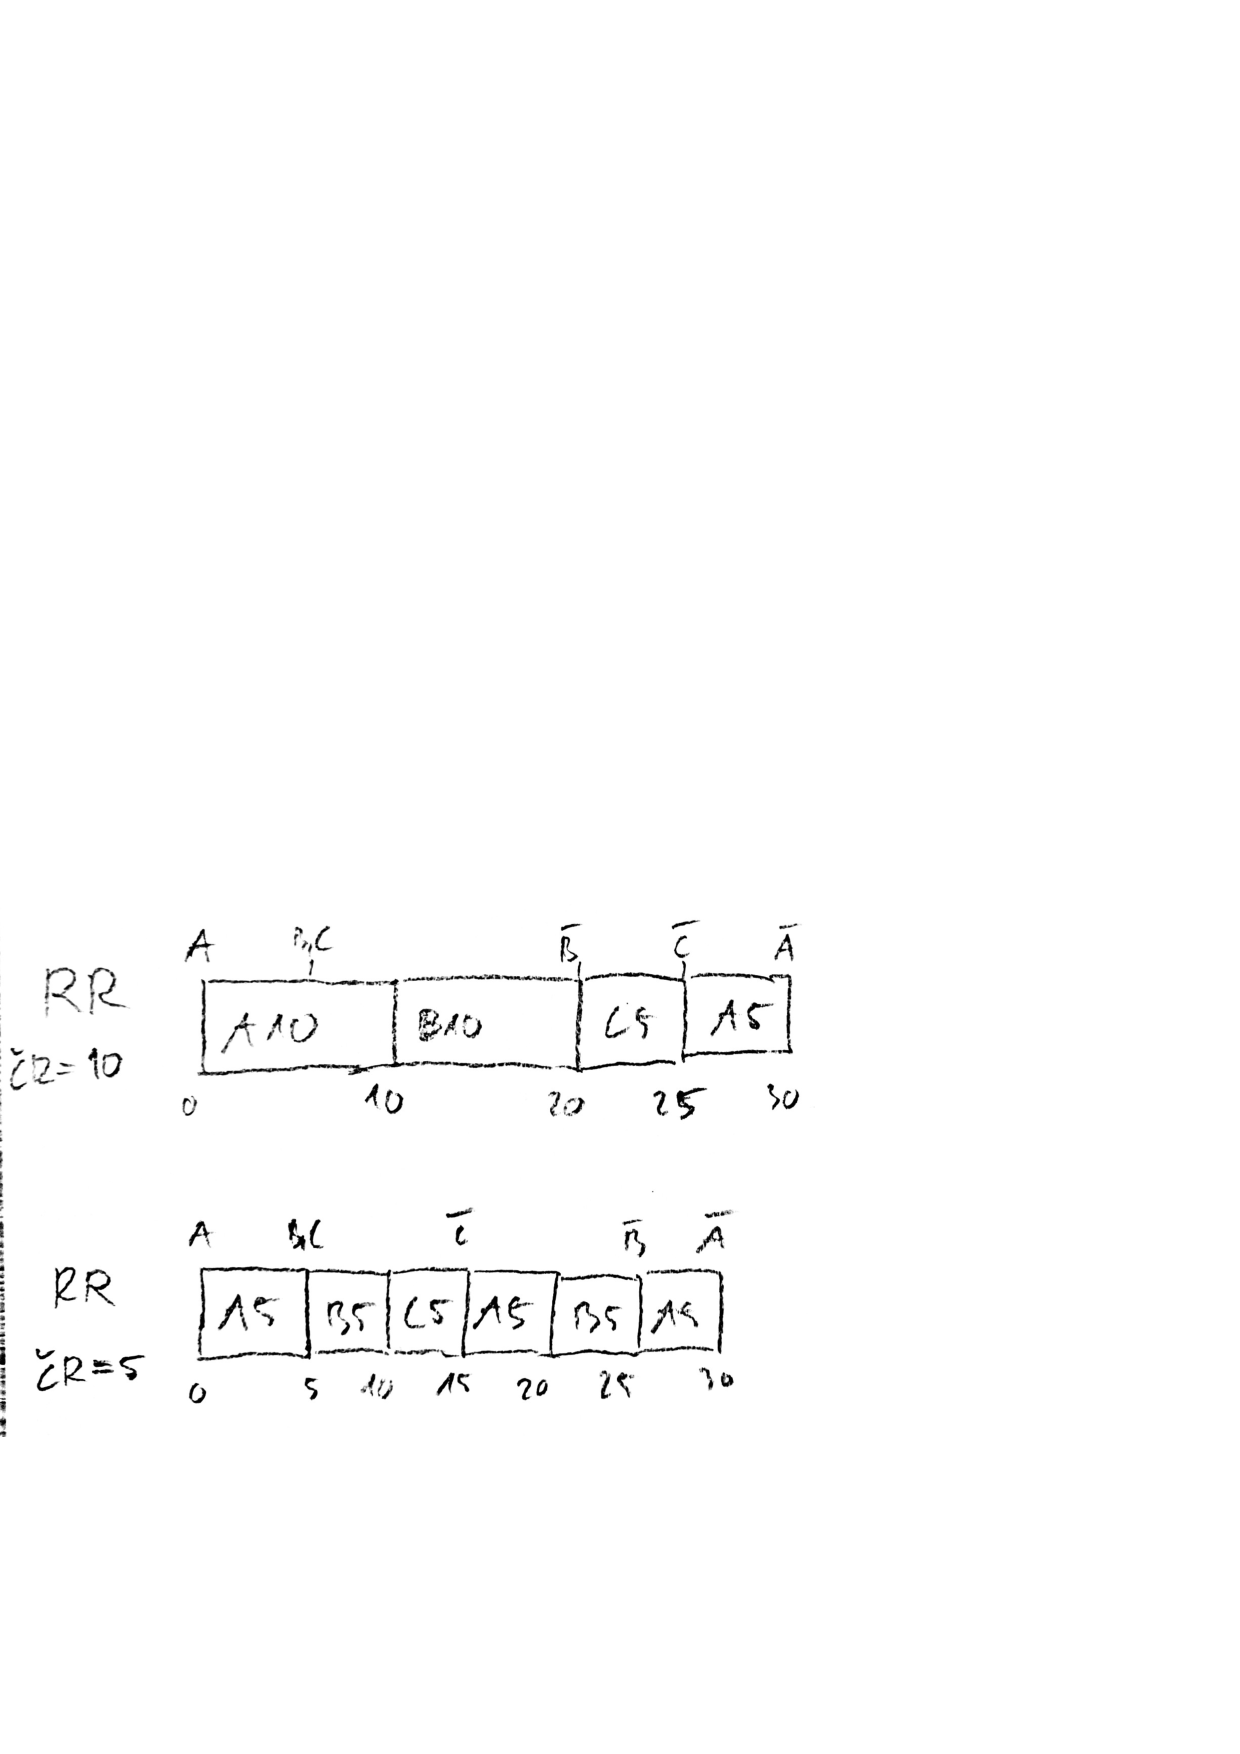
\includegraphics[width=.6\textwidth]{razvrscanje/1.5-RR.pdf}
\end{center}
}


\section{Efekt konvoja}

\intro{Naslednji dve nalogi sta namenjeni razlagi efekta konvoja na čas obdelave.}

\begin{Exercise}
Za razvrščanje procesov v dani tabeli uporabi optimalno razvrstitev glede na čas obdelave.
\par\vspace{5pt}
{\centering
\begin{tabular}{r|cccc}
	proces & A & B & C & D \\
	\hline
	trajanje & 7 & 2 & 19 & 6  \\
	čas prihoda & 0 & 0 & 0 & 0 \\
\end{tabular}\\}
\end{Exercise}
\ans{
OPT je SJF.
\begin{center}
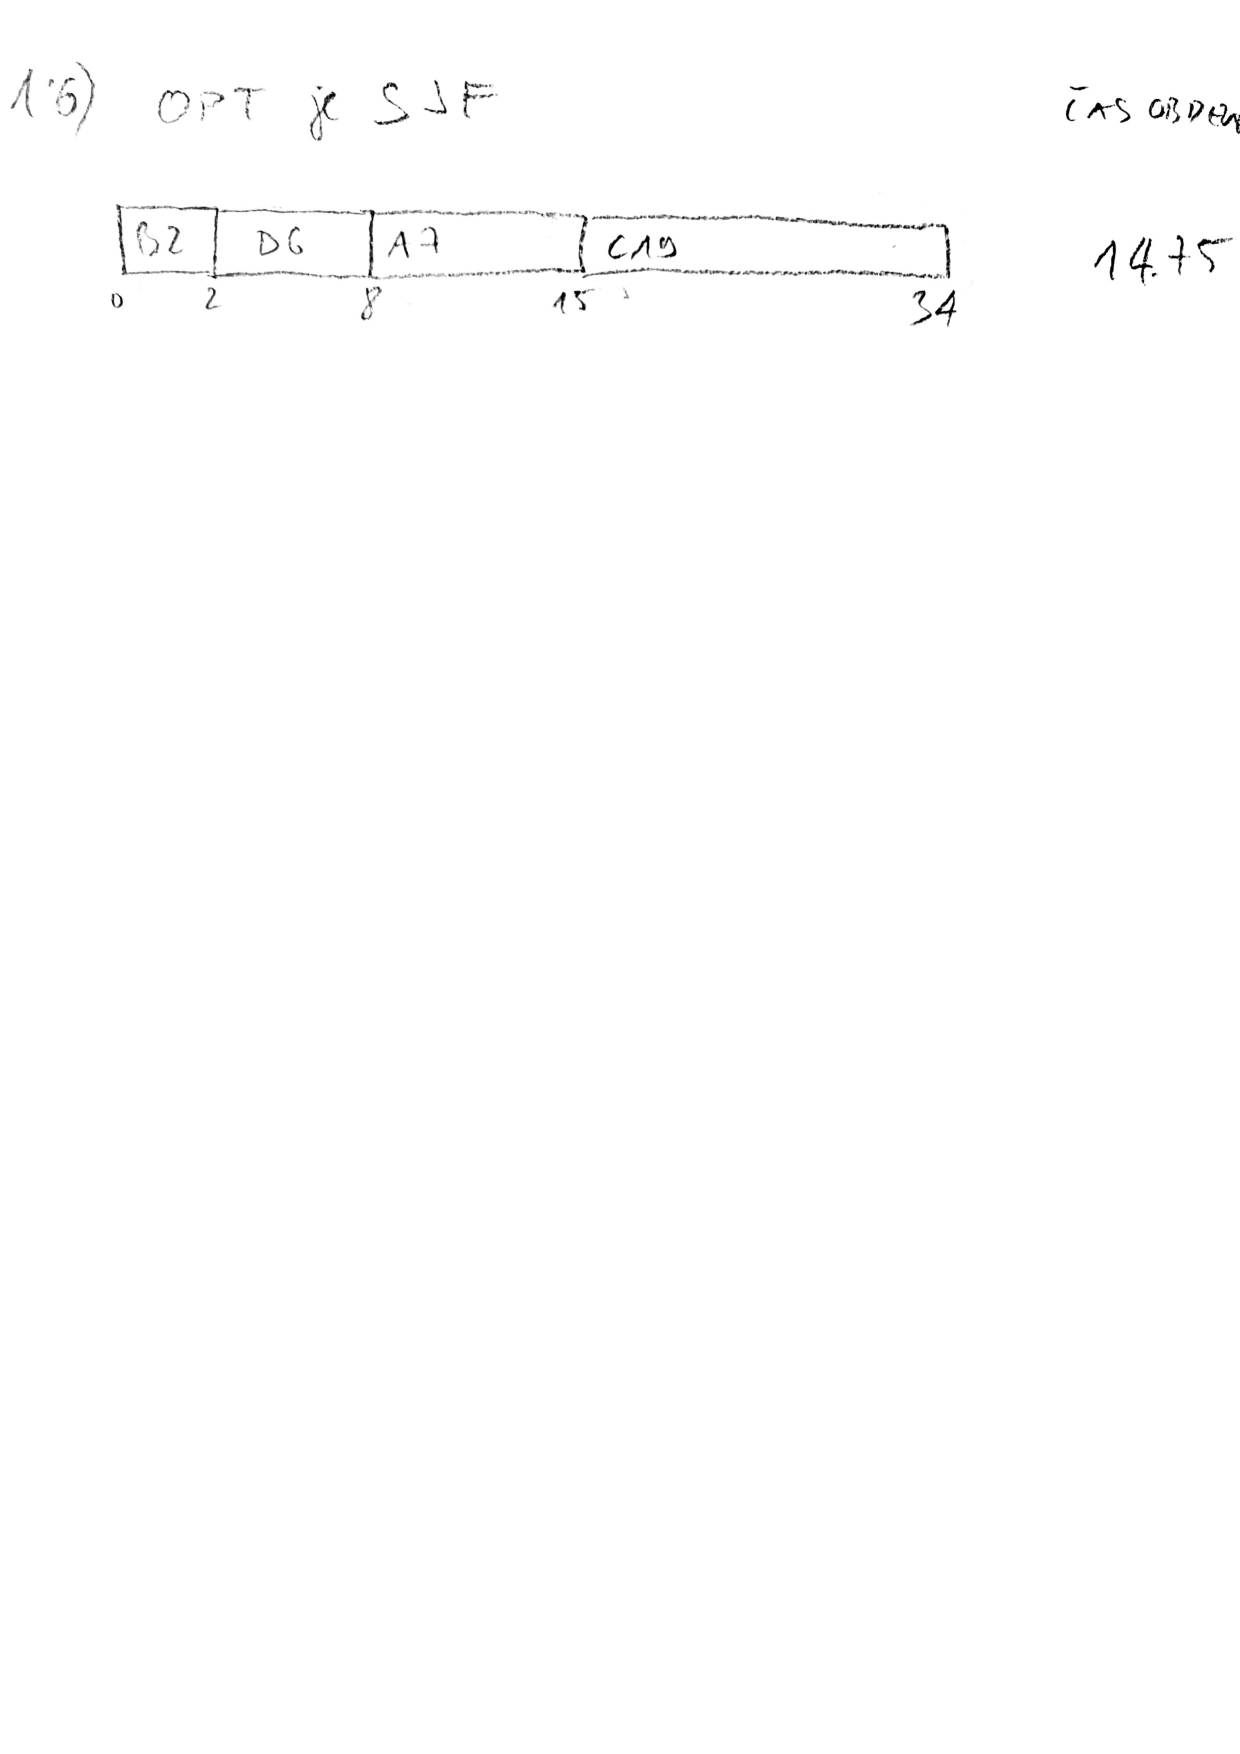
\includegraphics[width=.9\textwidth]{razvrscanje/1.6-OPT.pdf}\\
\begin{tabular}{c|cc|cc|cc}
proces & trajanje & prihod & začetek & odhod & odzivni čas & čas obdelave \\
\hline
A &   7 &  0 & 8 & 15 & 8 & 15 \\
B &   2 &  0 & 0 & 2 & 0 & 2 \\
C & 19 & 0 & 15 & 34 & 15 & 34 \\
D &   6 & 0 & 2 & 8 & 2 & 8 \\
\hline
& & & & & 6,25 & 14,75
\end{tabular}
\end{center}
}


\begin{Exercise}
Za razvrščanje procesov v dani tabeli uporabi algoritme FCFS, SJF in PSJF. V primeru dvoumnosti glede časa prihoda, procese razvrstimo leksikografsko.
\par\vspace{5pt}
{\centering
\begin{tabular}{r|cccc}
	proces & A & B & C & D \\
	\hline
	trajanje & 7 & 2 & 19 & 6  \\
	čas prihoda & 1 & 1 & 0 & 1 \\
\end{tabular}\\}
\end{Exercise}
\ans{
FCFS:
\begin{center}
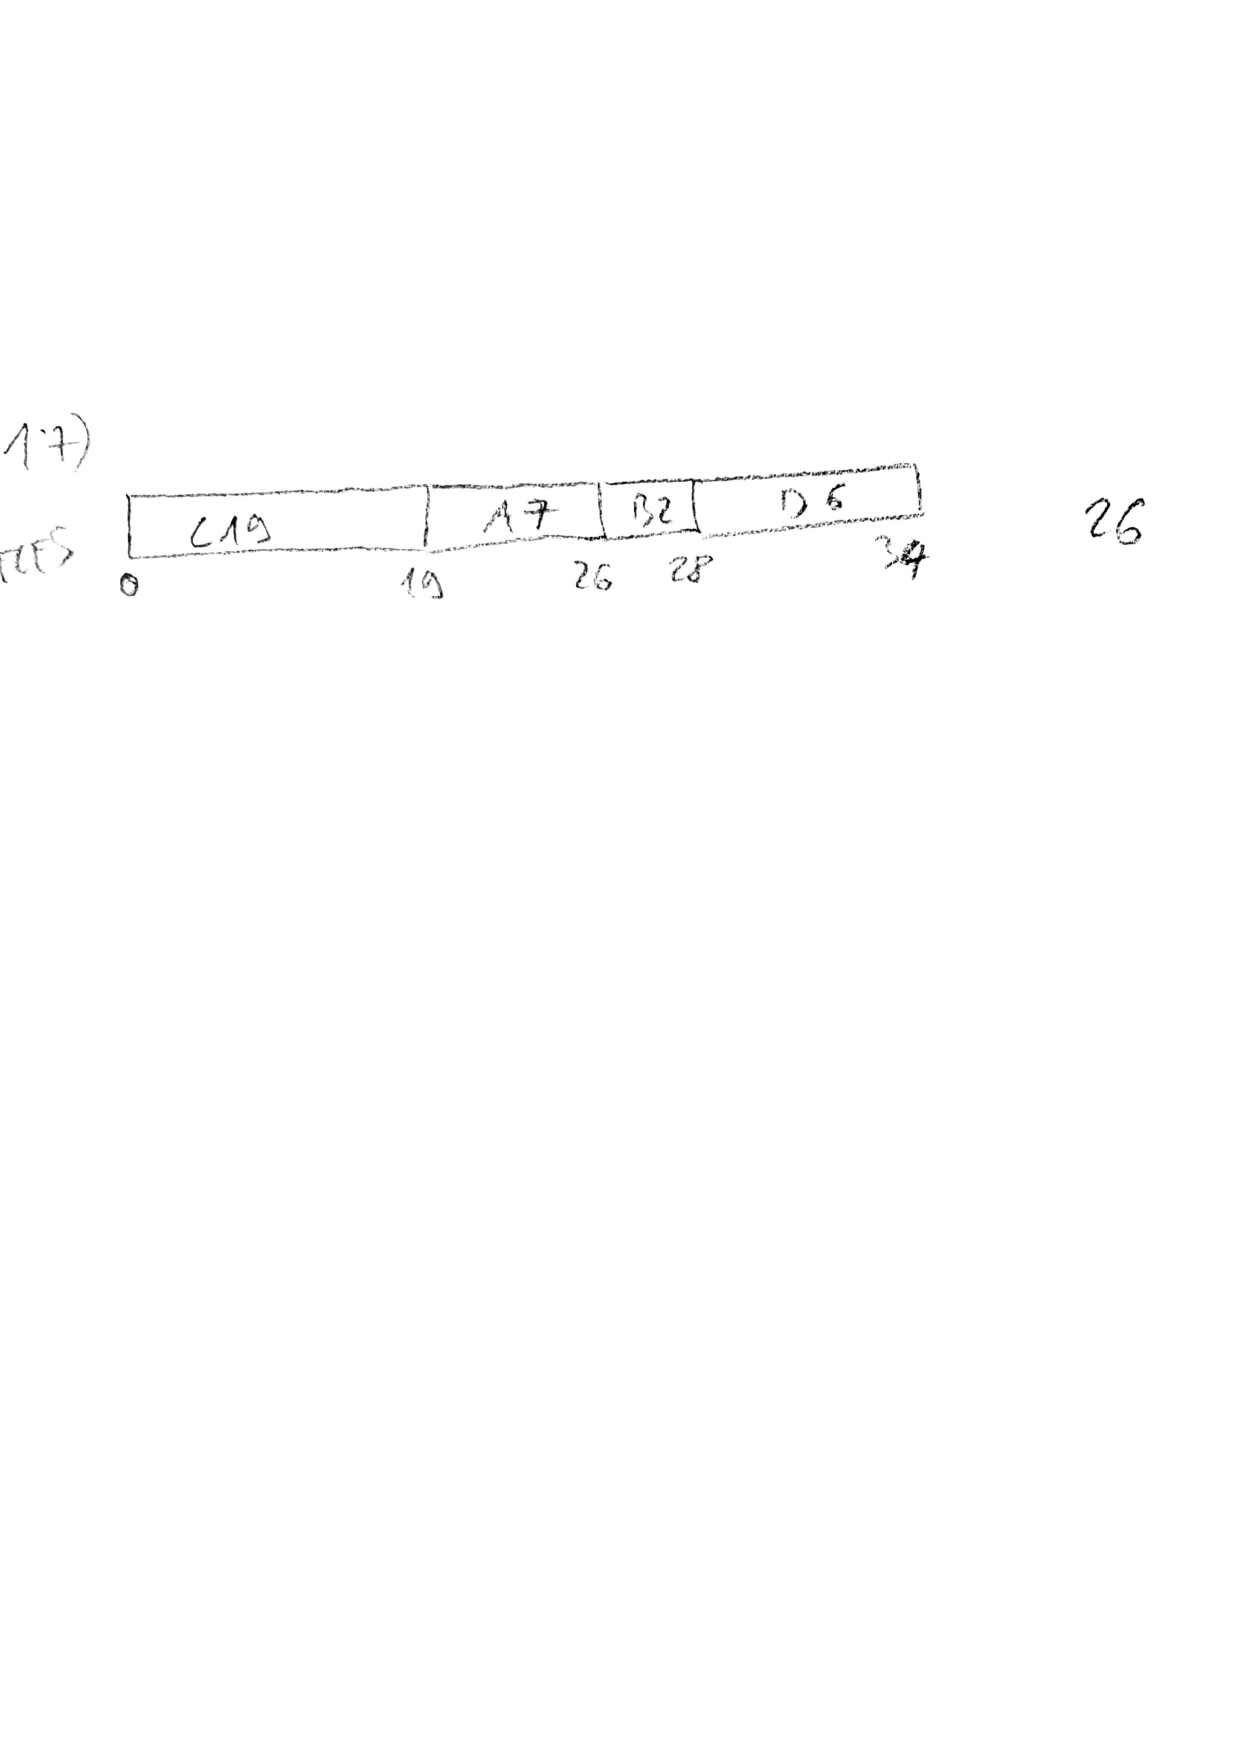
\includegraphics[width=.9\textwidth]{razvrscanje/1.7-FCFS.pdf}\\
\begin{tabular}{c|cc|cc|cc}
proces & trajanje & prihod & začetek & odhod & odzivni čas & čas obdelave \\
\hline
A &   7 &  1 & 19 & 26 & 18 & 25 \\
B &   2 &  1 & 26 & 28 & 25 & 27 \\
C & 19 & 0 &  0 & 19 & 0 & 19 \\
D &   6 & 1 & 28 & 34 & 27 & 33 \\
\hline
& & & & & 17,5 & 26
\end{tabular}
\end{center}
SJF:
\begin{center}
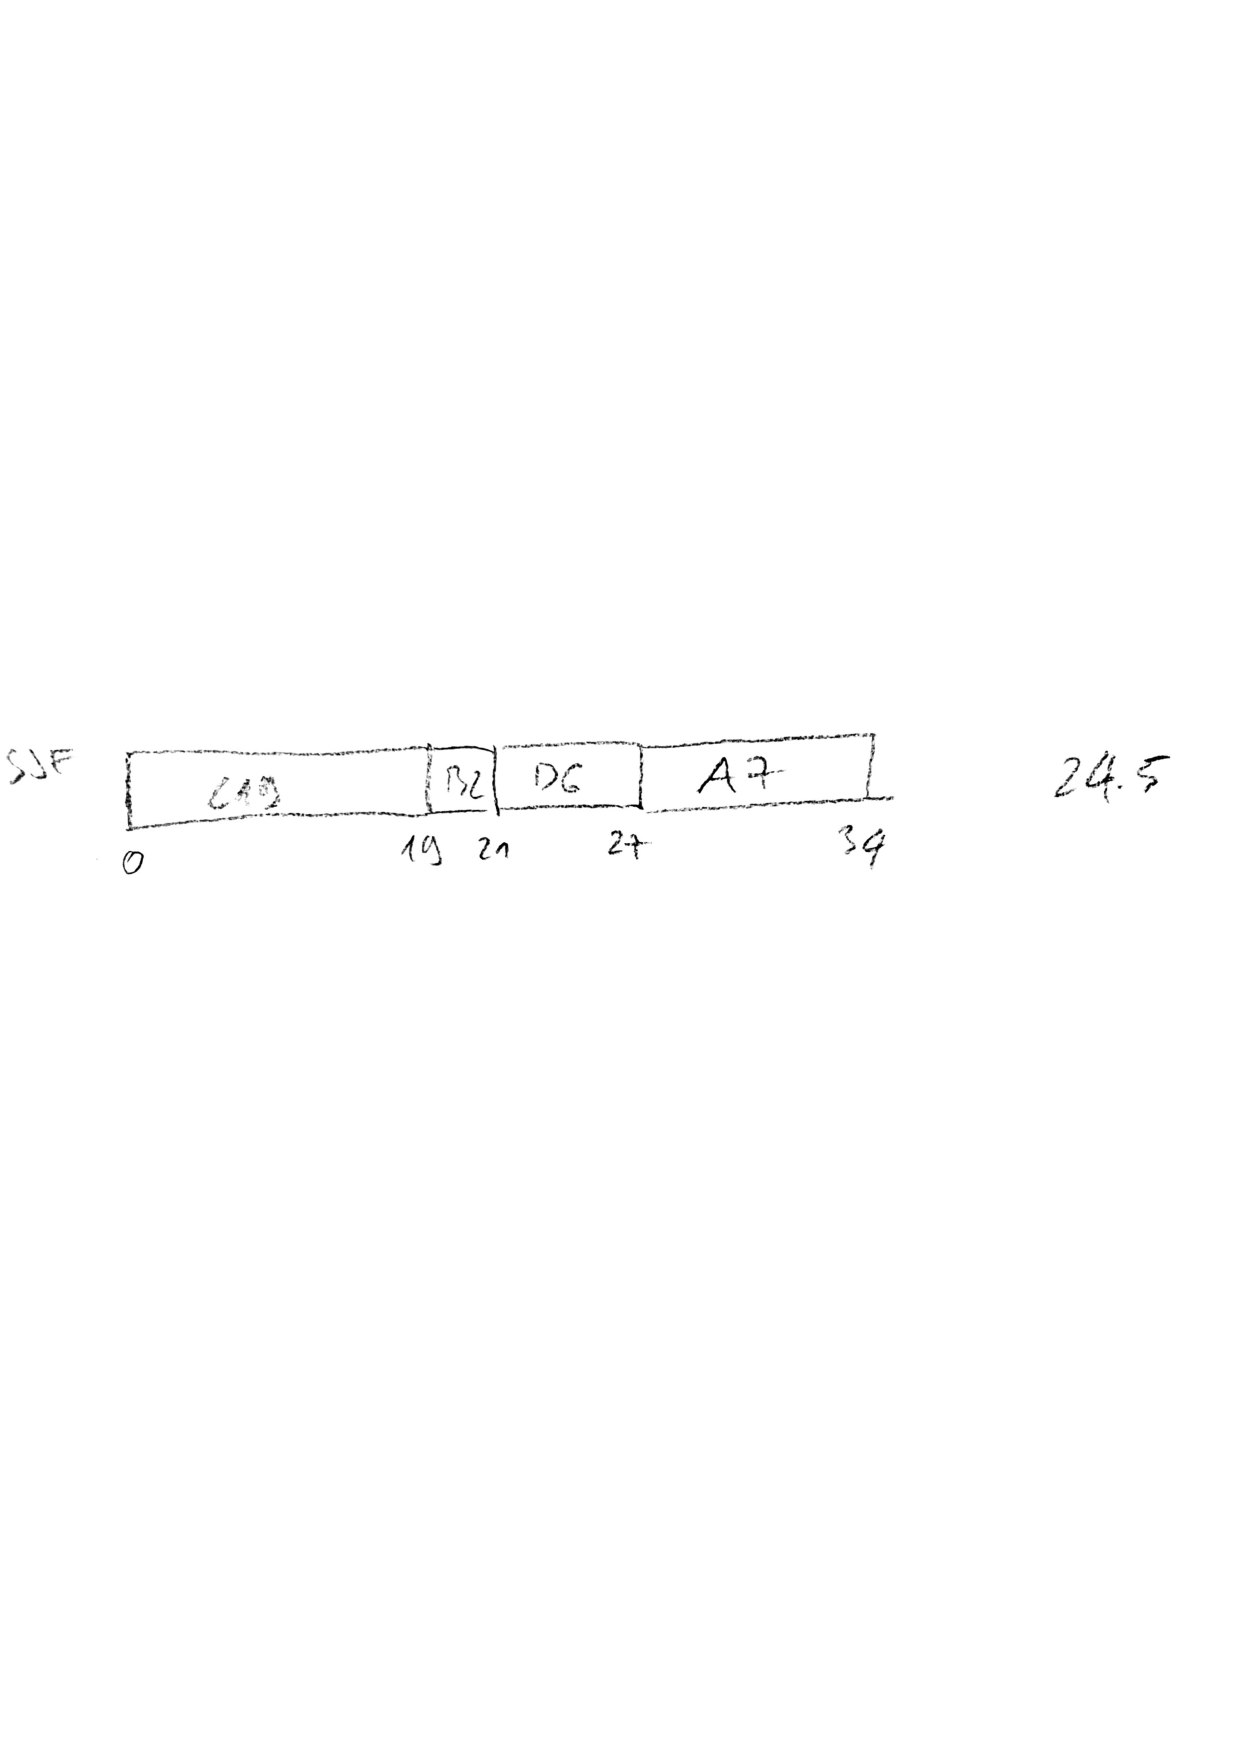
\includegraphics[width=.9\textwidth]{razvrscanje/1.7-SJF.pdf}\\
\begin{tabular}{c|cc|cc|cc}
proces & trajanje & prihod & začetek & odhod & odzivni čas & čas obdelave \\
\hline
A &   7 &  1 & 27 & 34 & 26 & 33 \\
B &   2 &  1 & 19 & 21 & 18 & 20 \\
C & 19 & 0 &  0 & 19 & 0 & 19 \\
D &   6 & 1 & 21 & 27 & 20 & 26 \\
\hline
& & & & & 16 & 24,5
\end{tabular}
\end{center}
PSJF:
\begin{center}
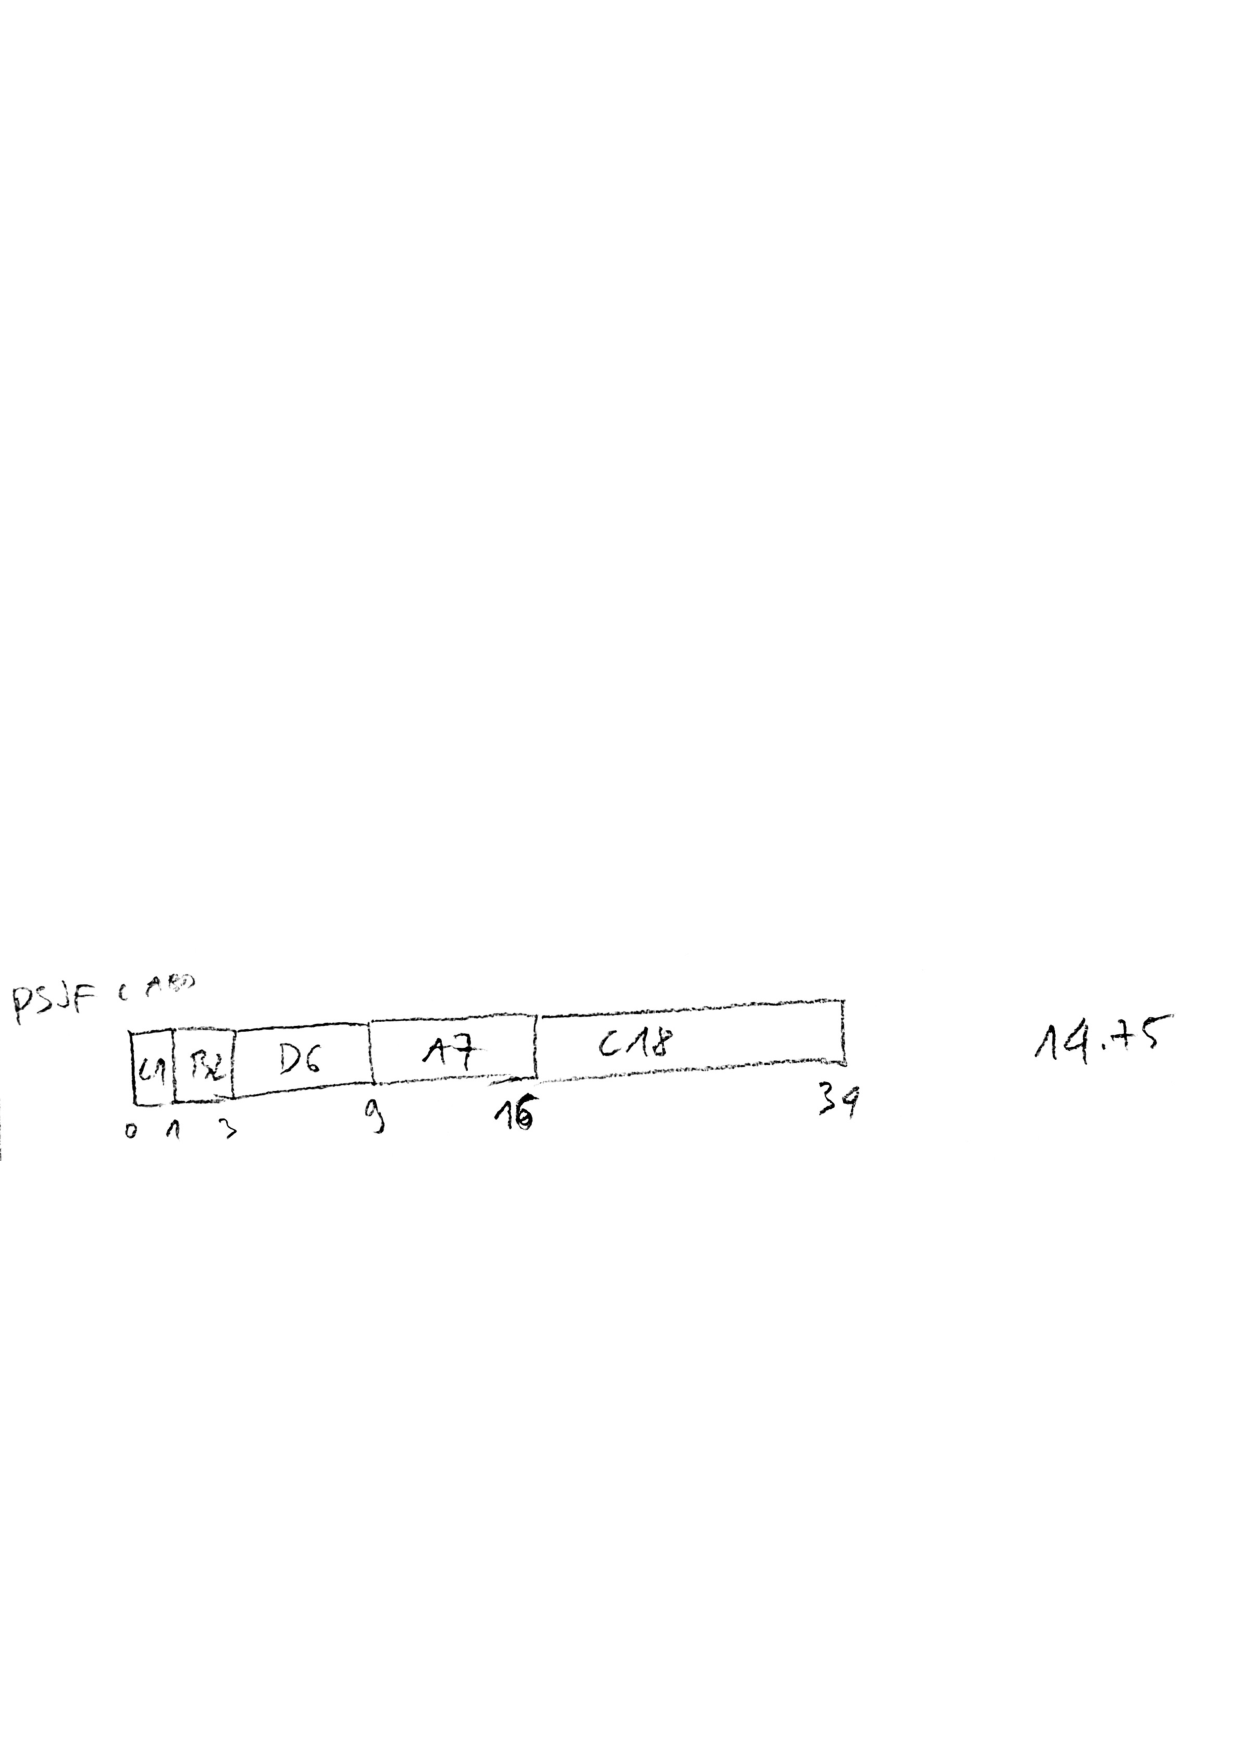
\includegraphics[width=.9\textwidth]{razvrscanje/1.7-PSJF.pdf}\\
\begin{tabular}{c|cc|cc|cc}
proces & trajanje & prihod & začetek & odhod & odzivni čas & čas obdelave \\
\hline
A &   7 &  1 & 9 & 16 & 8 & 15 \\
B &   2 &  1 & 1  & 3 & 0 & 2 \\
C & 19 & 0 & 0 & 34 & 0 & 34 \\
D &   6 & 1 & 3 & 9 & 2 & 8 \\
\hline
& & & & & 6,5 & 14,75
\end{tabular}
\end{center}
}

\section{Prednostna razvrščanja}


\begin{Exercise}
Za razvrščanje procesov v spodnji tabeli uporabi algoritem HPF, pri čemer
\begin{enumerate}
	\item uporabi sodelovano razvrščanje,
	\item uporabi prevzemno razvrščanje. 
\end{enumerate} 
\par\vspace{5pt}
{\centering
\begin{tabular}{r|ccc}
	proces & A & B & C \\
	\hline
	trajanje & 20 & 20 & 20  \\
	čas prihoda & 0 & 10 & 20 \\
	prioriteta & 1 & 2 & 3 \\
\end{tabular}\\}
\end{Exercise}
\begin{Answer}
Sodelovalno HPF razvrščanje:
\begin{center}
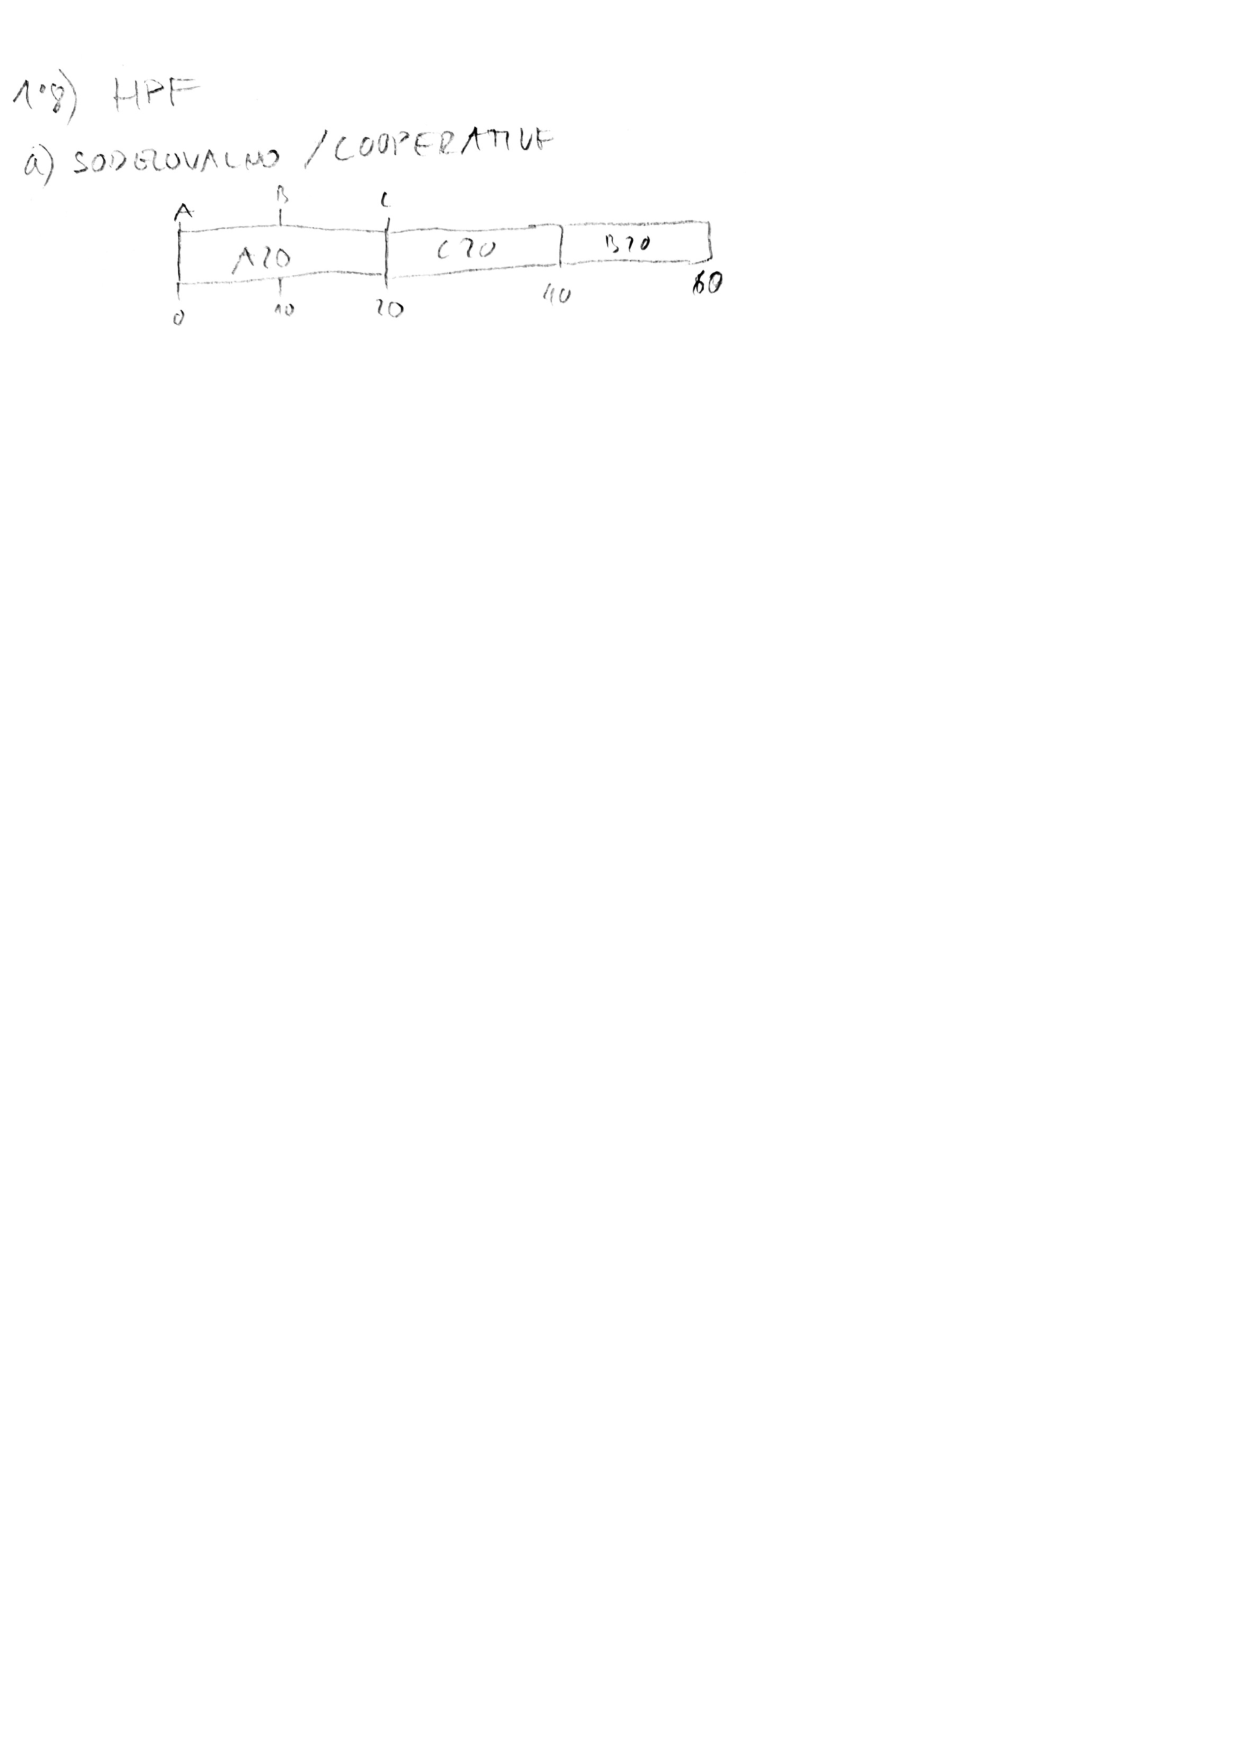
\includegraphics[width=.9\textwidth]{razvrscanje/1.8-HPF-cooperative.pdf}\\
\begin{tabular}{c|ccc|cc|cc}
proces & trajanje & prihod & prioriteta & začetek & odhod & odzivni čas & čas obdelave \\
\hline
A & 20 &  0 &  1 &   0 & 20 & 0 & 20 \\
B & 20 & 10 & 2 & 40 & 60 & 30 & 50 \\
C & 20 & 20 & 3 & 20 & 40 & 0 & 20 \\
\hline
& & & & & & 10 & 30
\end{tabular}
\end{center}
Prevzemno HPF razvrščanje:
\begin{center}
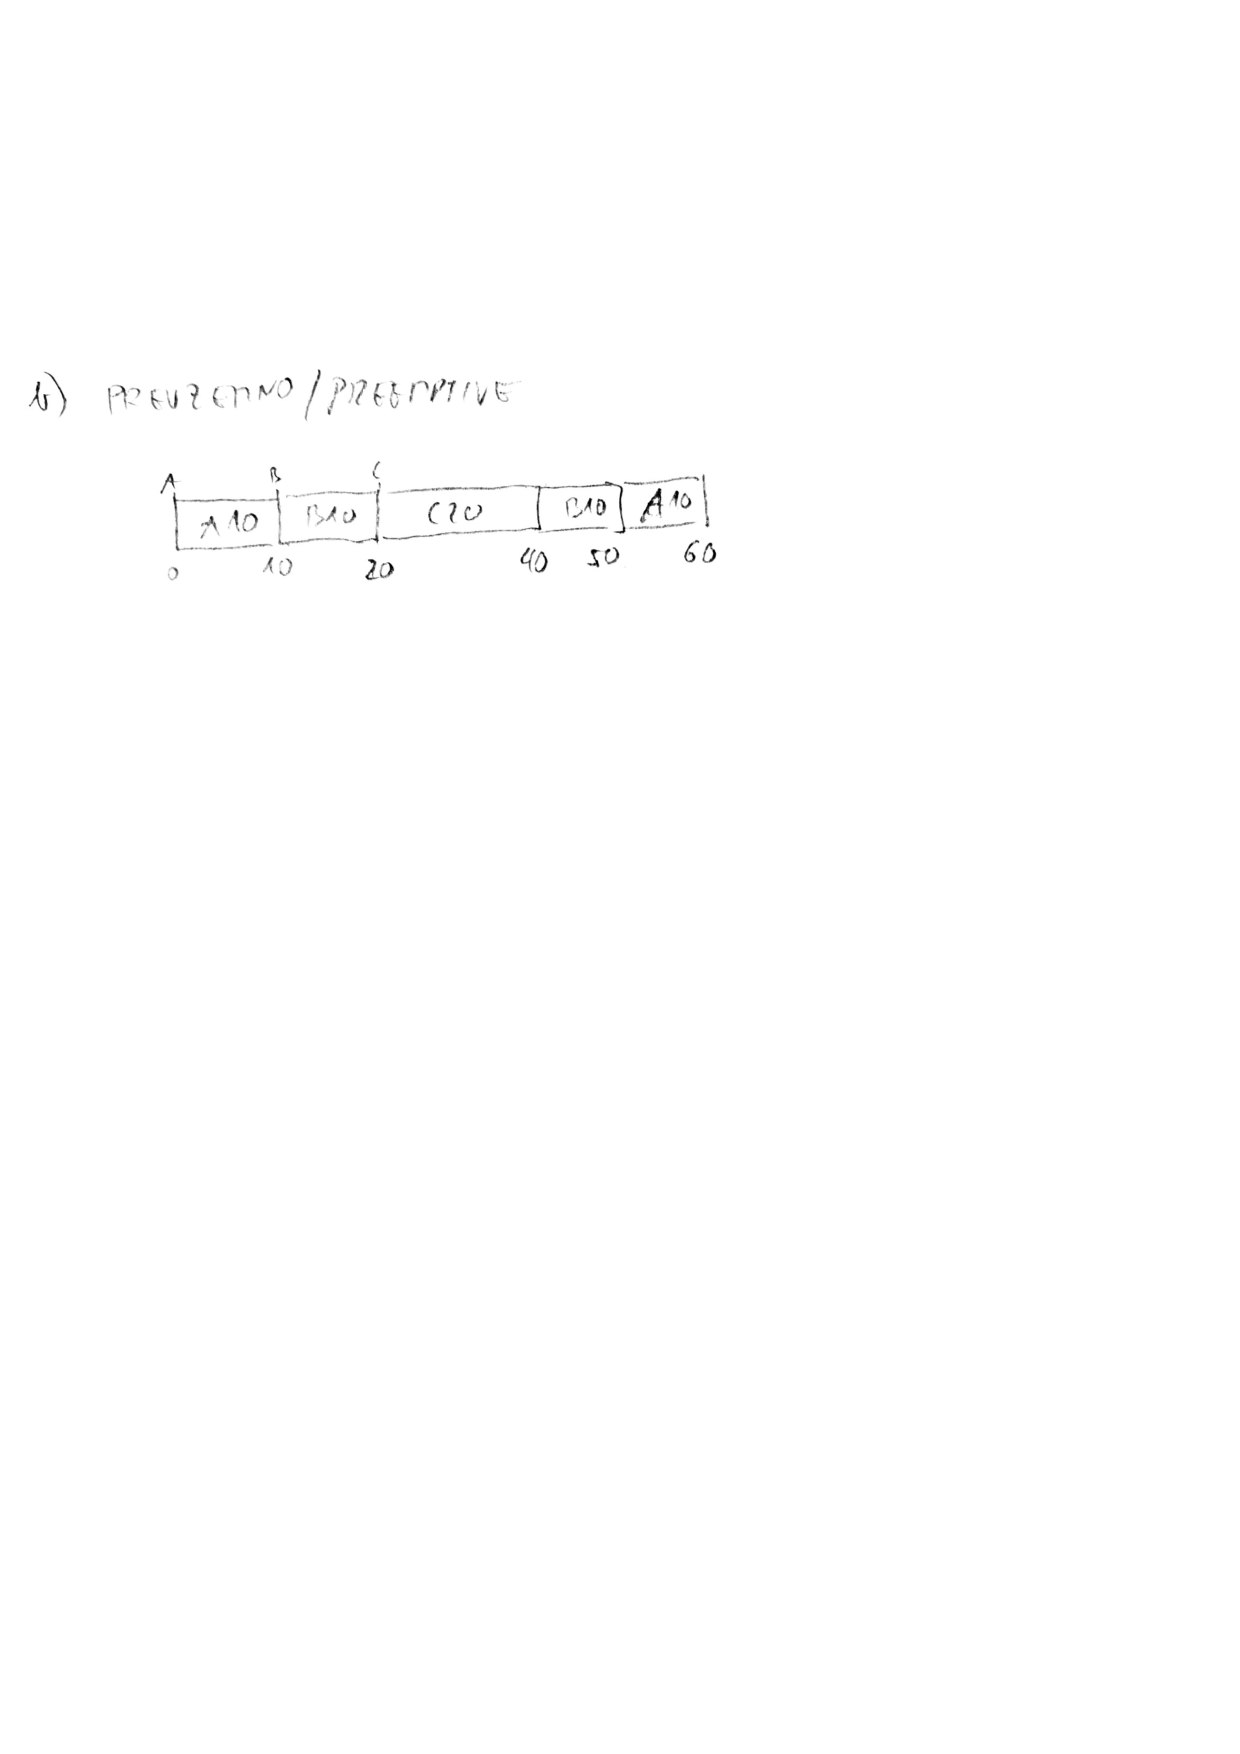
\includegraphics[width=.9\textwidth]{razvrscanje/1.8-HPF-preemptive.pdf}\\
\begin{tabular}{c|ccc|cc|cc}
proces & trajanje & prihod & prioriteta & začetek & odhod & odzivni čas & čas obdelave \\
\hline
A & 20 &  0 &  1 &   0 & 60 & 0 & 60 \\
B & 20 & 10 & 2 & 10 & 50 & 0 & 40 \\
C & 20 & 20 & 3 & 20 & 40 & 0 & 20 \\
\hline
& & & & & & 0 & 40
\end{tabular}
\end{center}
\end{Answer}


\exe{Procesi A, B in C imajo 10, 20 in 40 prepustnic zaporedoma. Razvrščevalni algoritem je izbral prepustnice št. 15, 5, 10, 42, 9, 66. Zapiši vrstni red, ki ustreza izbranimi prepustnicam. Prepustnice številčimo od 0 naprej.}
\ans{Vrstni red: B,A,B,C,A,C
\begin{center}
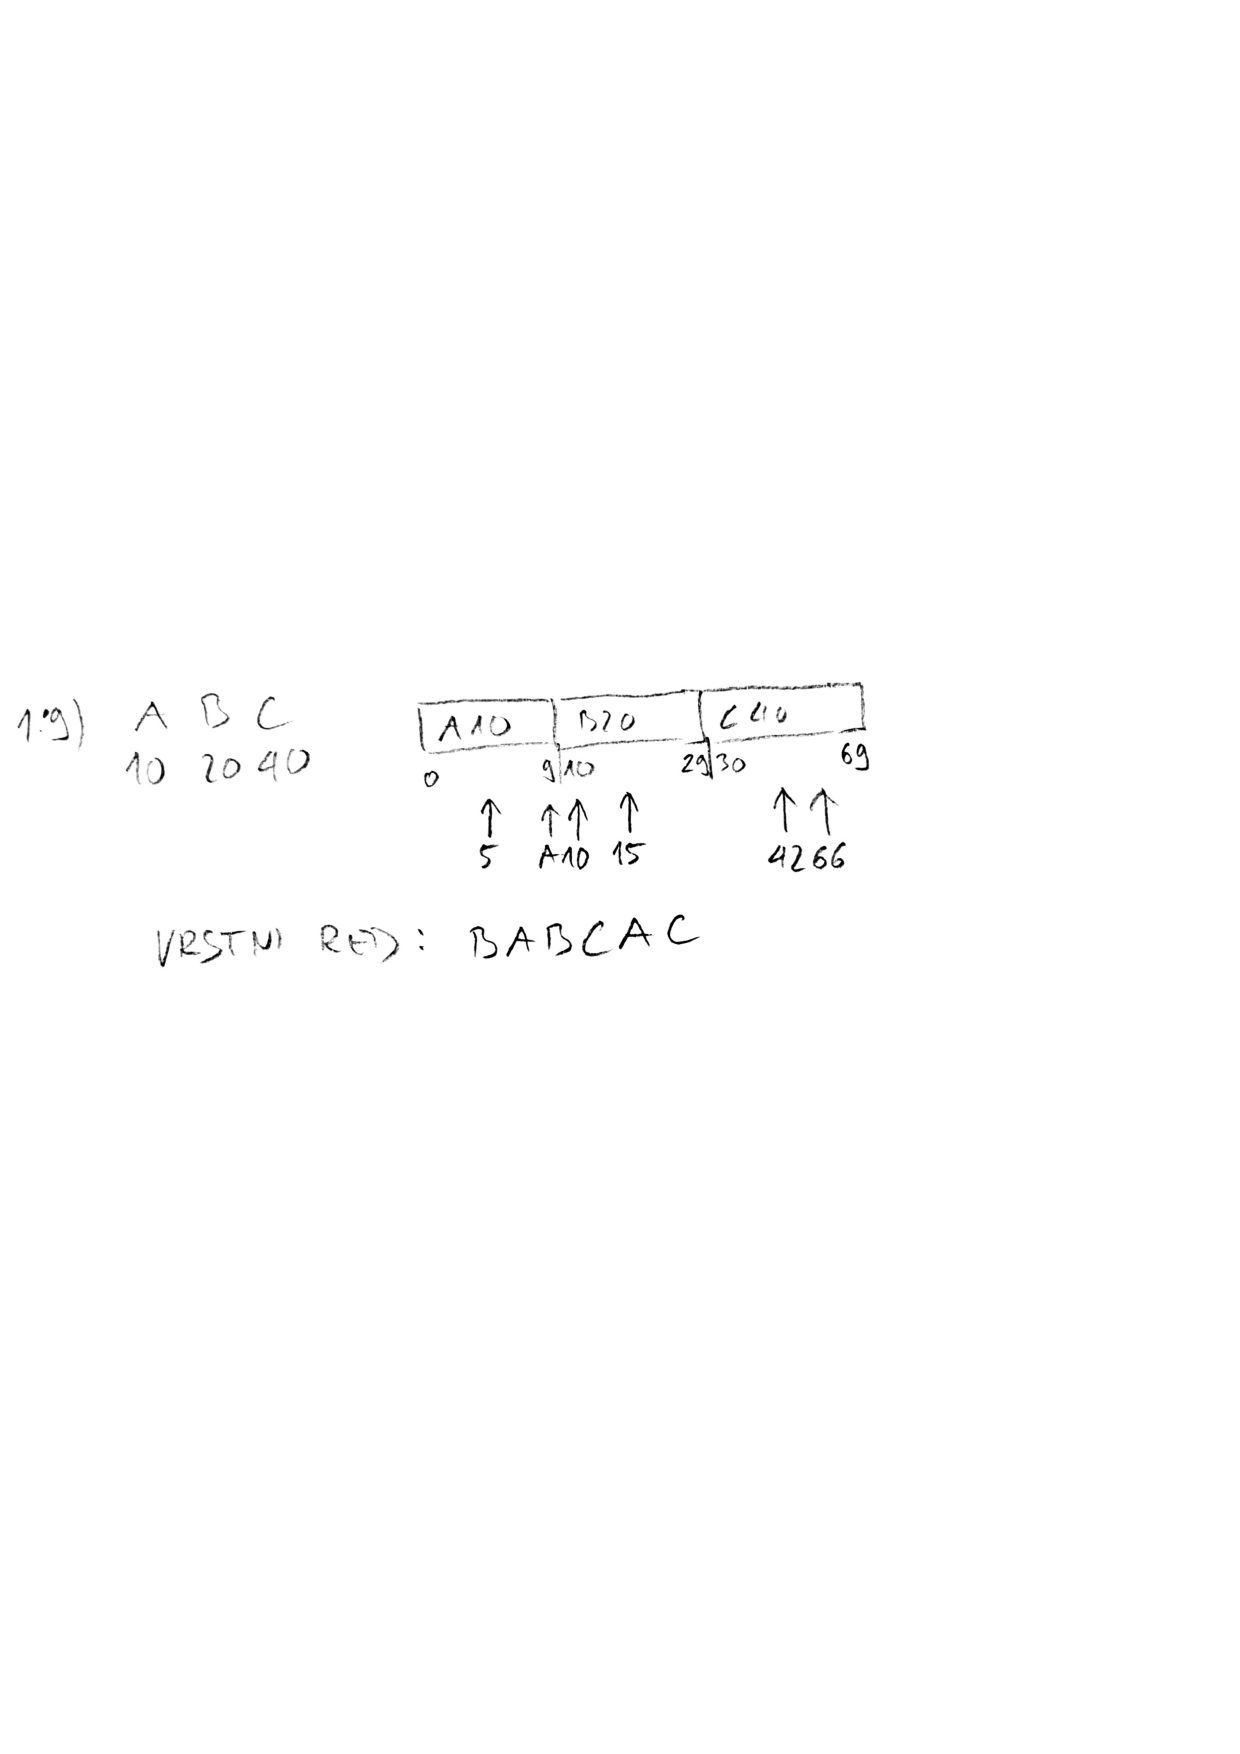
\includegraphics[width=.9\textwidth]{razvrscanje/1.9-tickets.pdf}
\end{center}
}


\exe{Procesi A, B in C imajo dolžine korakov 10, 15 in 30 zaporedoma. Uporabi koračno razvrščanje in zapiši prvih 10 izbranih procesov, pri čemer predpostavljaj \vic{neskončno} trajanje procesov.}
\ans{A,B,C,A,B,A,A,B,C, nato se vse skupaj ponovi neskončnokrat. Časovna rezina je lahko poljubna.
\begin{center}
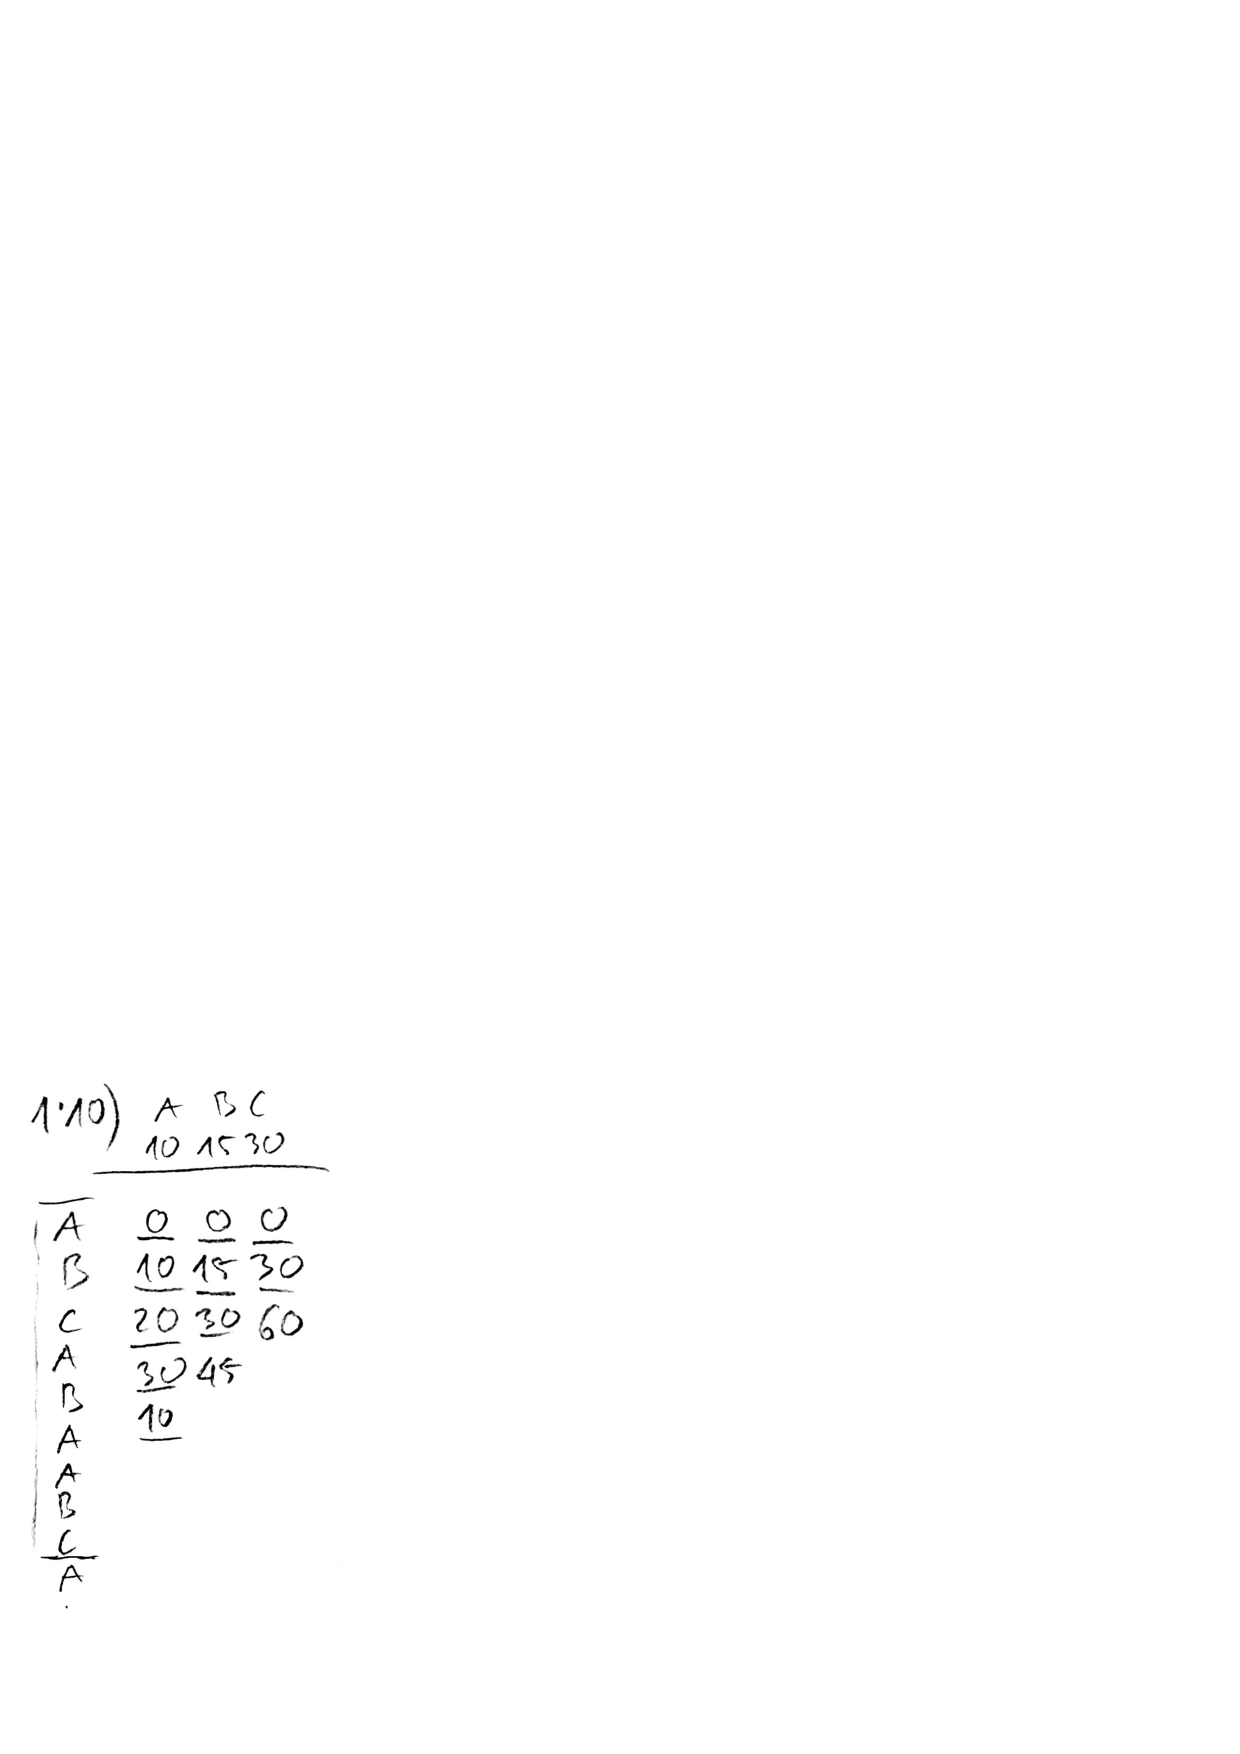
\includegraphics[width=.4\textwidth]{razvrscanje/1.10-stride.pdf}
\end{center}
}


\exe{Procesi A, B in C imajo dolžine korakov 10, 15 in 30 zaporedoma, njihovo trajanje pa je 40, 20, 30, zaporedoma. Uporabi koračno razvrščanje s časovno rezino 10 in zapiši prvih 10 izbranih procesov.}
\ans{A,B,C,A,B,A,A,C,C
\begin{center}
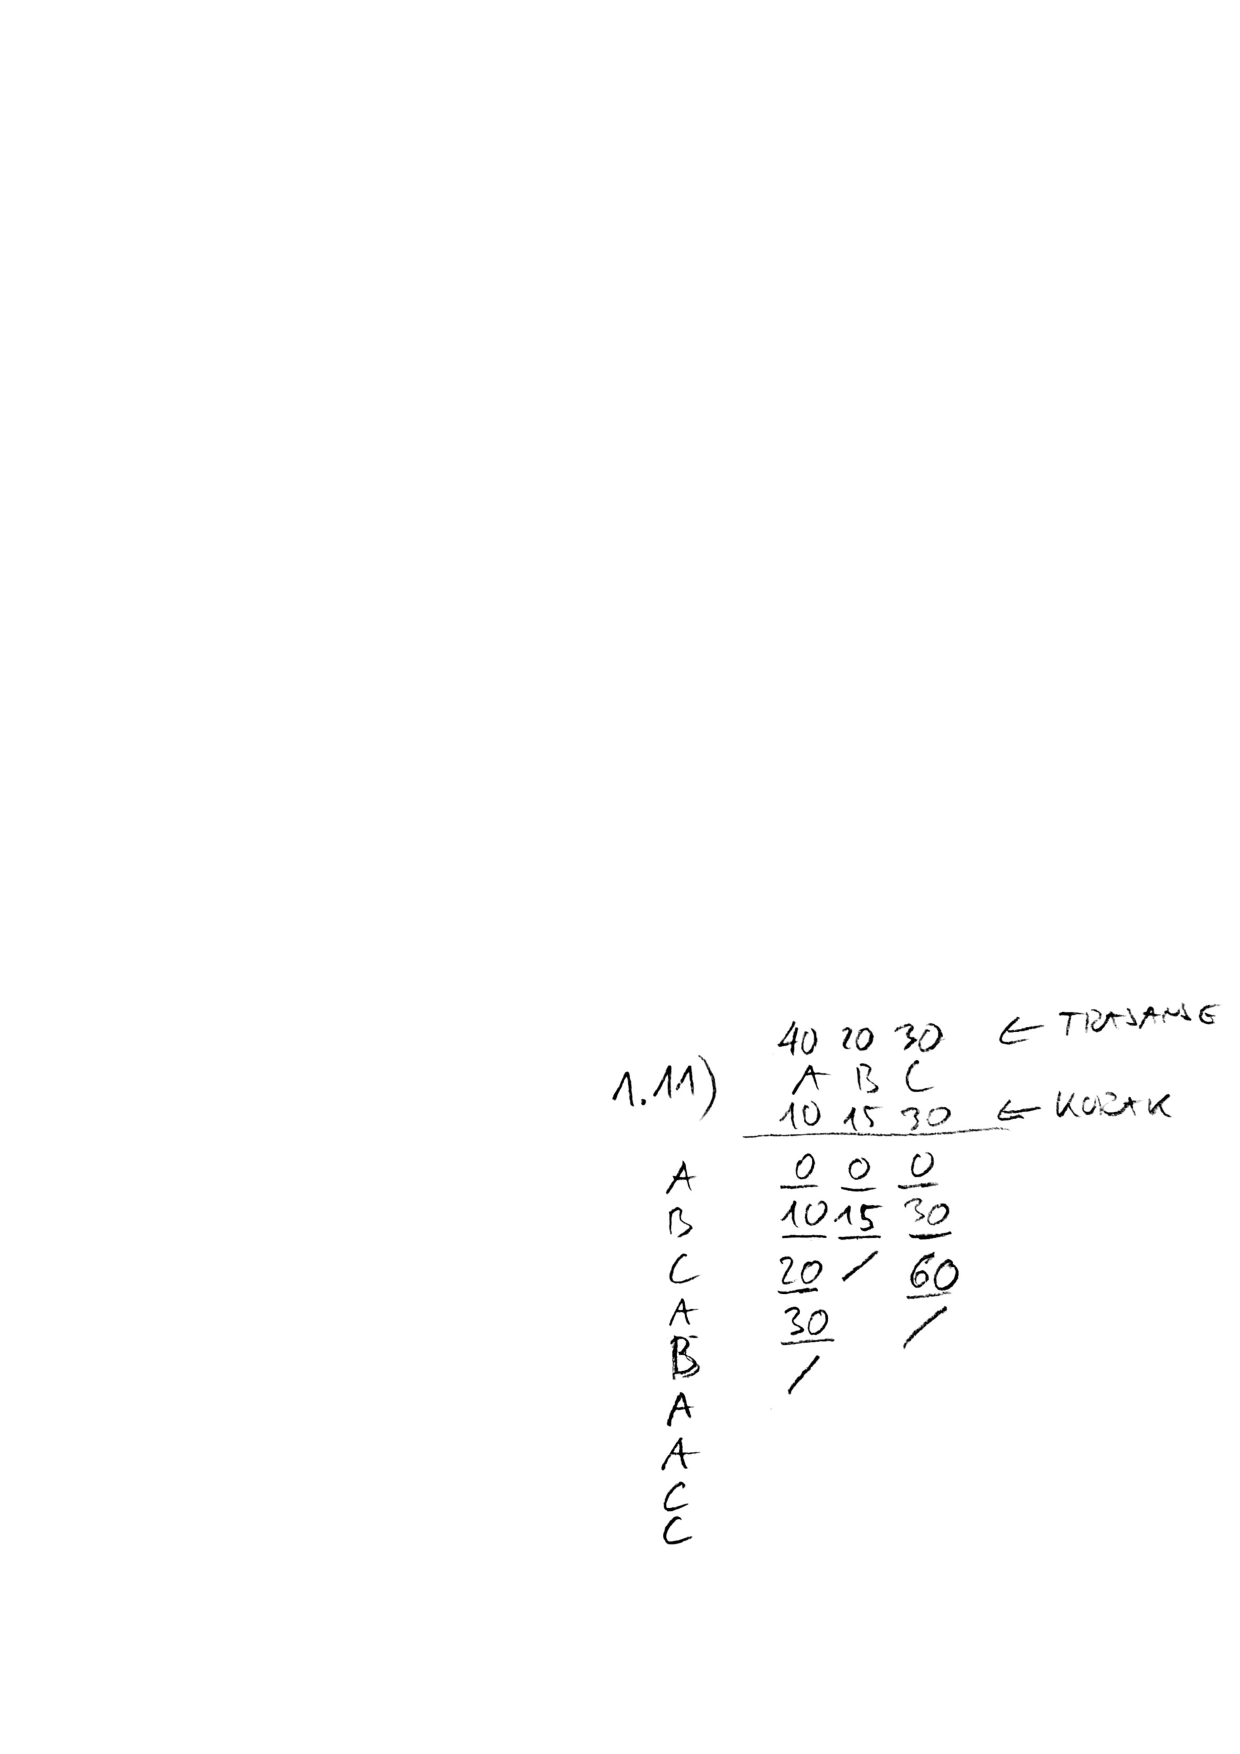
\includegraphics[width=.5\textwidth]{razvrscanje/1.11-stride.pdf}
\end{center}
}


\section{Ocenjevanje trajanja procesov}

\intro{Trajanje procesa ocenjujemo po formuli
$$ T_i = \alpha\cdot t_i + (1-\alpha)\cdot T_{i-1}, $$
kjer je $\alpha$ faktor pozabljanja, $t_i$ zadnje trajanje procesa in $T_i$ zadnja ocena trajanja. Nova ocena trajanja procesa pa je $T_{i+1}$. Začetno oceno označimo s $T_0$.}


\begin{Exercise}
Naj bo $\alpha=0.5$ faktor pozabljanja in $T_0=5$ začetna ocena trajanja procesa. Dopolni tabelo z ocenami trajanja procesov:
\par
{\centering
	\begin{tabular}{c|cccc}
		$i$    & 1 & 2 & 3 & 4 \\ 
		\hline
		$t_i$ & 11 & 4 & 2 & 20 \\
		$T_i$ &  &  &  &  \\
	\end{tabular}\\
}
\end{Exercise}
\ans{
	\begin{tabular}{c|cccc}
	$i$    & 1 & 2 & 3 & 4 \\ 
	\hline
	$t_i$ & 11 & 4 & 2 & 20 \\
	$T_i$ & 8 & 6 & 4 & 12 \\
	\end{tabular}\\
}


\begin{Exercise}
Naj bo $\alpha=0.2$ faktor pozabljanja in $T_0=10$ začetna ocena trajanja procesa. Dopolni tabelo z ocenami trajanja procesov:
\par
{\centering
	\begin{tabular}{c|cccc}
	$i$    & 1 & 2 & 3 & 4 \\ 
	\hline
	$t_i$ & 10  & 15 & 16 & 22\\
	$T_i$ & & & & \\
	\end{tabular}\\
}
\end{Exercise}
\ans{
\begin{tabular}{c|cccc}
	$i$    & 1 & 2 & 3 & 4 \\ 
	\hline
	$t_i$ & 10  & 15 & 16 & 22\\
	$T_i$ & 10 & 11 & 12 & 14 \\
\end{tabular}\\
}


\section{Namigi in rešitve izbranih nalog}

\shipoutAnswer

\chapter{Sistemski klici}

\section{Iz lupine v C}

Pri nalogah tega tipa je podan ukaz za lupino bash. Potrebno pa je sprogramirati program v jeziku C, ki naredi enako kot dani ukaz. Pri tem
\begin{itemize}
	\item ukaze vgrajene v lupino sprogramiramo s pomočjo sistemskih klicev
	\item zunanje ukaz zaženemo preko \id{fork()} \& \id{exec()}
	\item uporabljamo le V/I funkcije brez medpomnilnika, torej \id{open()}, \id{read()}, \id{write()} in \id{close()}
	\item uporaba funkcij, ko sta npr. \id{system()} in \id{popen()} ni dovoljena
\end{itemize}


\begin{Exercise}
Napiši program v programskem jeziku C, ki naredi enako kot naslednji ukaz v lupini bash.
\begin{enumerate}
	\item \code{mkdir house \&\& touch mouse}
	\item \code{cat <mouse | head -42}
\end{enumerate}
\end{Exercise}




\end{document}
